% XeLaTeX can use any Mac OS X font. See the setromanfont command below.
% Input to XeLaTeX is full Unicode, so Unicode characters can be typed directly into the source.

% The next lines tell TeXShop to typeset with xelatex, and to open and save the source with Unicode encoding.

%!TEX TS-program = xelatex
%!TEX encoding = UTF-8 Unicode

\documentclass[11pt]{article}
\usepackage{geometry,authblk,multicol,amsmath}
\usepackage[square,numbers,sort&compress]{natbib}
\usepackage[textsize=small]{todonotes}                % See geometry.pdf to learn the layout options. There are lots.
\geometry{letterpaper}                   % ... or a4paper or a5paper or ... 
%\geometry{landscape}                % Activate for for rotated page geometry
%\usepackage[parfill]{parskip}    % Activate to begin paragraphs with an empty line rather than an indent
\usepackage{graphicx}
\usepackage{amssymb}
\usepackage{booktabs}
\usepackage{multirow}
\usepackage{url}

% Will Robertson's fontspec.sty can be used to simplify font choices.
% To experiment, open /Applications/Font Book to examine the fonts provided on Mac OS X,
% and change "Hoefler Text" to any of these choices.

\usepackage{fontspec,xltxtra,xunicode}
\defaultfontfeatures{Mapping=tex-text}
\setromanfont[Mapping=tex-text]{Times New Roman}
\setsansfont[Scale=MatchLowercase,Mapping=tex-text]{Gill Sans}
\setmonofont[Scale=MatchLowercase]{Andale Mono}

\title{Combinatorial Mixture Models for Single Cell Assays}
\author[1]{Greg Finak}
\author[2]{SC De Rosa}
\author[1]{Raphael Gottardo}

\affil[1]{Vaccine and Infectious Disease Division, Fred Hutchinson Cancer Research Center (FHCRC), Seattle, WA}
\affil[2]{HIV Vaccine Trials Network, Fred Hutchinson Cancer Research Center (FHCRC), Seattle, Wa}
\date{\today}                                       

\begin{document}
\maketitle

\begin{abstract}
Immunological endpoints in vaccine trials are measured through a variety of assays that  provide single--cell measurements of multiple genes and proteins in specific immunological cell populations. %intracellular or cell surface proteins, or mRNA expression levels of genes in single cells from specific immunological cell populations. 
Using single--cell data, we consider the problem of identifying subjects where these cell populations exhibit differential responses under different experimental conditions.  
%While these measurements are usually continuous, they are often discretized and analyzed as counts of single cells. 
For example, in the intracellular cytokine staining assay from flow cytometry, individual cells are classified as either positive or negative for a marker based on a predetermined threshold.  %One such assay is the intracellular cytokine staining assay that
The assay is used to assess an individual's immune response to a vaccine by measuring the number of antigen--specific cells  producing different cytokines in different T--cell subpopulations in response to different antigen stimulations.  Individuals whose T--cells exhibit increased production of a cytokine in response to stimulation are termed ``positive'' for that cytokine, and multiple such ``positivity calls'' are used to identify vaccine responders. 
%Cells are classified as cytokine positive or negative and the resulting The cell counts are used to identify experimental conditions leading to an increase in cytokine producing cells. The ICS assay is generally used to identify ``vaccine responders''. These are individuals whose immune system produces significantly more cytokine positive cells in response to antigen stimulation than at baseline. The rarity of these cell populations makes maximizing the sensitivity and specificity of the assay a primary concern. The standard approach to analyze such data, Fisher's exact test, is problematic for two reasons. It can be overly conservative in detecting true differences for small counts, and the data generally do not meet the assumptions of the test. Specifically, the total cell counts across conditions are generally not fixed since these are generated by independent experiments.  
Here we present a framework based on mixtures of Beta--binomial or Dirichlet--Multinomial distributions for analyzing count data derived from such single--cell assays.  Our method models cellular responses in a marker--specific manner, treating the responding and non--responding observations as separate components in the model. Cell counts from the different experimental conditions are modelled independently, while sharing information across responding and non--responding observations through empirical Bayes priors in order to increase the sensitivity and specificity of positivity calls. We compare our method against Fisher's exact test and show how it can be extended to model multivariate (multiple markers) cellular responses. In simulations and in HIV vaccine trial data we find that our method has higher sensitivity and specificity than Fisher's exact test for positivity calls. 
% simultaneously, sharing information across observations using empirical Bayes methods. The model represents the responder and non-responder observations as separate components in the model, stimulated and unstimulated cell counts are modelled independently. Using simulations and real--world vaccine trial data, we show that our model increases the sensitivity and specificity for positivity calls in ICS assays compared to Fisher's exact test. 
\end{abstract}

\section{Introduction}
Single--cell assays are an important tool in immunology, providing a functional and phenotypic snapshot of the immune system at a given time. These assays typically measure multiple variables simultaneously on individual cells in a heterogeneous mixture such as whole blood. These variables are used to classify individual cells in the mixture into more homogeneous sub--populations based on phenotypic or functional differences. Such single--cell assays are used for immune monitoring of disease, vaccine research, and diagnosis of haematological malignancies~\cite{Altman:1996wf,Betts:2006dw,Inokuma:2007tn}.

A motivating example from vaccine research is the flow cytometric intracellular cytokine staining (ICS) assay, which is used to identify individuals whose immune system responds to a vaccine. Upon vaccination, antigen in the vaccine is taken up and presented to CD4 or CD8 T--cels via antigen presenting cells. While not all T--cells can recognize all antigens, those that recognize antigens in the vaccine become \emph{activated} and produce a variety of cytokines, further promoting the immune response. After activation, this antigen--specific subpopulation proliferates and can persist in the immune system for some time providing \emph{memory} that can more rapidly recognize the same antigen again in the future\cite{McKinstry:2010ei}. These antigen--specific T--cell subpopulations a very small fraction of the total number of CD4 and CD8 T--cells. The ICS assay measures the number of antigen--specific T--cells in whole blood by measuring cytokine production in response to activation following stimulation by an antigen that was present in the original vaccine. Individual cells are labelled using fluorescently conjugated antibodies against phenotypic markers (CD3, CD4, and CD8) and functional markers (cytokines) of the cell subpopulations of interest~\cite{Horton:2007tsa,DeRosa:2004wp,Betts:2006dw}. A sufficiently large number of cells must be collected to ensure that the rare cell populations can be detected. Subsequently, each individual cell is classified as either positive or negative for each maker based on predetermined thresholds, then the number of cells matching each subpopulation phenotype is counted. These counts are compared between antigen stimulated and unstimulated samples from an individual to identify significant differences. Assessing a broad T cell response to a vaccine is particularly important in HIV vaccine trials, where the search for immune correlates of protection against HIV progression and infection is ongoing~\cite{Plotkin:2010ve,Horton:2007tsa,Kim:2010fw, Bendall:2011wf}.

The ICS assay in flow cytometry is just one example of the applications of single--cell technologies to immunology. Single--cell gene expression technologies such as Fluidigm are enabling researchers to measure the expression of 96 genes in 96 single cells from a homogeneous population sorted by flow cytometry\cite{Jang:2011uj}. This technology has been used to identify signatures of immune cell sub--populations that correlate with different types of vaccine~\cite{Flatz:2011jb}. To date, published analysis of Fluidigm data ignore cells where transcripts are undetected, focusing solely on continuous gene expression measurements. However, the proportion of single cells expressing individual genes also carries information and should be evaluated.

Although there is no standard approach to analyzing ICS assay data current methods range from ad--hoc rules based on log--fold changes, to permutation tests based on Hotelling's T$^2$ statistics, to exact tests of 2x2 contingency tables (e.g., Fisher's exact test)~\cite{Trigona:2003,Sinclair:2004hs,Horton:2007tsa,Nason:2006dx}. These methods generally test pairwise combinations of markers, raising questions of appropriate multiple testing adjustments, or they perform global tests of significance on multiple markers resulting in decreased power to detect small changes in subsets of cytokines~\cite{Proschan:2009ks,Nason:2006dx}. 


%on a per--cytokine basis to identify observations where the number of cytokine producing cells is greater in the stimulated than the control data Problems with Fisher's exact when the test assumptions are not met have been reviewed in the literature~\cite{Proschan:2009ks}. In the context of single--cell assay data the assumption of fixed margins is not satisfied since the observations for treatment and control conditions arise from independent experiments, thus the p--values from Fisher's exact test are incorrect. More importantly, Fisher's exact test does not share information across observations, resulting in low power when counts are small. 

The framework developed in this paper addresses these issues explicitly. We present a combinatorial mixture model framework for the analysis of single--cell assay data where multivariate measurement are made on individual cells. The model is used to identify observations where a significant difference exists between paired treatment and control samples with respect to the number of cells expressing  different combinations of proteins, genes, or other measured properties of the cells. Importantly, our approach shares information across observations by means of prior distributions on the responding, stimulated samples and the non--responding samples thereby increasing sensitivity and specificity to detect responding cell populations. The cell counts from the stimulated and unstimulated experiments are modelled independently, and different combinations of markers are represented as different mixture components in the framework. This approach allows us to omit certain combinations of markers that are not observable (i.e., two cytokines may never be co--expressed), or to explicitly represent combinations that are of interest (i.e., we can explicitly represent and test for a difference in a pair of cytokines in an experiment measuring many cytokines). This is a flexible approach that avoids the some of the drawbacks of global tests when only a few of the many measured markers show differences~\cite{Nason:2006dx}.

\section{Data structure and notation} 
We analyzed two data sets from two different immunological single--cell assays typically used in vaccine trials, one flow cytometry data set, and one single--cell gene expression data set.

\textit{Flow cytometry}: This ICS data is from a phase--I (safety and efficacy) trial of an adenoviral vector vaccine in individuals without prior immunity, measuring four cytokines in two cell populations from 20 individuals at two time points (zero and 28 days post--vaccination, see Supplementary Information~\ref{supp:data} for details)~\cite{Peiperl:2010ej}. The statistical analysis of responder and non--responder calls in the published trial is described in the original manuscript and outlined in the supplementary information (Supplementary Information~\ref{supp:statpublished})~\cite{Peiperl:2010ej}. The goal of this data set was to assess response rates of CD4 and CD8 T--cell populations to different antigens.

\textit{Fluidigm single--cell gene expression}: This is a single--cell gene expression data set of flow--sorted CD8 T--cells from sixteen individuals. The T--cells from blocks of four individuals were stimulated with different antigens, gene expression measured at the single--cell level and compared to paired, unstimulated controls. 

In the remainder of the paper, we use the following notation to describe our model. We observe cell counts from $P$ subjects in two conditions (stimulated and unstimulated). Each cell can either be positive or negative for a marker. We let $i$ index the subjects and $k$ index the cytokines. The subscripts $s$,$u$ refer to the cell counts from stimulated and unstimulated conditions, respectively. The total number of cells is denoted by $N$, and given in our model, while $n$, the number of positive cells is part of the observe data. Thus for a given cytokine, $N_{si}$ denotes the total number of cells collected for subject $i$ in the stimulated condition and $n_{si}$ denotes how many of those cells were cytokine positive. Similarly, $N_{ui}$, $n_{ui}$ represent the total, and cytokine positive cell counts in the unstimulated condition for the same subject. For each cytokine and each stimulation, given the total cell counts, the observed data is a matrix of size $2 \times P$, where the $i$'th row is a subject, $\mathbf{y}_i = <n_{si},n_{ui}>$. 

\section{Differential expression with one marker}
The data for a single marker can be represented in contingency table form:

\begin{table}[ht]
\centering
\parbox{0.8\linewidth}{
\caption{2 x 2 contingency table of counts for cytokine positive and cytokine negative events between stimulated and unstimulated conditions}\label{tab:twobytwo}
\centering
\begin{tabular}{rrr}

  \hline
\multicolumn{1}{l}{}&
\multicolumn{2}{c}{Cytokine}\\
 & Negative & Positive \\ 
  \hline
Stimulated &   $N_{si} - n_{si}$ &   $n_{si}$ \\ 
Unstimulated &   $N_{ui}-n_{ui}$ &   $n_{ui}$ \\ 
   \hline
\end{tabular}
}
\end{table}
We consider a marker to be differentially expressed between conditions if the number of cells in the stimulated samples is significantly different from the number of cells in the control sample. The model is described below.

\subsection{Beta--Binomial Model for One Marker}
The positive cell counts for stimulated and unstimulated samples from the same individual are modelled as  binomial random variables.
\begin{align}
(n_{si}|p_{ui}) \sim \mathrm{Bin}(N_{si},p_{ui});\text{ }& (n_{ui}|p_{ui}) \sim \mathrm{Bin}(N_{ui},p_{ui})\label{eq:null};&\text{if $i$ is a non--responder}\\
(n_{si}|p_{si}) \sim \mathrm{Bin}(N_{si},p_{si});\text{ }& (n_{ui}|p_{ui}) \sim \mathrm{Bin}(N_{ui},p_{ui});&\text{if $i$ is a responder}\label{eq:alternate}
 \end{align}
 
Where $p_{si}$, $p_{ui}$ are the unobserved proportions. Model~\eqref{eq:null} represents the \textit{null} hypothesis where there is no difference between the stimulation and the control, and thus no difference between the proportion of cytokine positive cells in stimulated and control samples. Model~\eqref{eq:alternate} represents the  alternative hypothesis where there is a difference in cytokine response between the stimulation and the control, and thus a difference in the proportion of cells between stimulated and control samples. In the case of no response, the counts for the stimulated and unstimulated samples are independent draws from the same  binomial distribution. 

\subsection{Prior}
Our model shares information across responders and non--responders, respectively. This is done by placing Beta priors on the $p_{si}$, $p_{ui}$, across subjects:
 
 \begin{align}
 p_{si} &\sim \mathrm{Beta}(\alpha_s,\beta_s);&
 p_{ui} &\sim \mathrm{Beta}(\alpha_u, \beta_u)\label{eq:prior}
 \end{align}

Additional sharing of information is done through the $\alpha_u, \beta_u$ hyper--parameters, which are common for the null and alternative models. 
%If $p_{si}=p_{ui}$ we assume that $\alpha_s=\alpha_u$ and $\beta_s=\beta_u$, thus sharing the hyper--parameters between the null and alternative model for the unstimulated samples, such that $\beta_u,\alpha_u$ hyper--parameters are equal for both the stimulated and unstimulated models. Given this formulation, the posterior probability of the data given that it is generated by model \eqref{eq:null}, is:
\subsection{Posetrior}
\subsubsection{Null Model}
Given the above formulation, the posterior for the null model is Beta--binomial, with marginal likelihood (integrating out $p_u$):

 \begin{align}
  	\mathrm{L}(\alpha_u,\beta_u|\mathbf{y})
	&=\prod_{i=1}^P\binom{N_{si}}{n_{si}}\binom{N_{ui}}{n_{ui}}\frac{\mathrm{B}(n_{si}+n_{ui}+\alpha_u,N_{si}-n_{si}+N_{ui}-n_{ui}+\beta_u)}{\mathrm{B}(\alpha_u,\beta_u)}\label{eq:model1post}
%	\intertext{Integrating out the proportions gives the marginal log--likelihood.}
%	\begin{split}
%	\mathcal{L}(\alpha_u,\beta_u|\mathbf{y})=\sum_{i=1}^P\left[\log{\binom{N_{si}}{n_{si}}}+\log{\binom{N_{ui}}{n_{ui}}}+\right.\\
%	\left.\log{\left(\mathrm{B}(n_{si}+n_{ui}+\alpha_u,N_{si}-n_{si}+N_{ui}-n_{ui}+\beta_u)\right)}\right]-P\log\left(\mathrm{B}(\alpha_u,\beta_u)\right)\label{eq:model1MLL}
%	\end{split}
 \end{align} 
 \subsubsection{Alternative Model - Unconstrained}
 If the data is generated by model~\eqref{eq:alternate} then we have  $p_s\ne p_u$, and the marginal likelihood of the alternative is:
\begin{align}
	\begin{split}
\mathrm{Pr}(y_i|\alpha_u,\beta_u,\alpha_s,\beta_s) =\binom{N_{ui}}{n_{ui}} \binom{N_{si}}{n_{si}}\frac{\mathrm{B}(n_{ui}+\alpha_u,N_{ui}-n_{ui}+\beta_u)}{\mathrm{B}(\alpha_u,\beta_u)}\frac{\mathrm{B}(n_{si}+\alpha_s,N_{si}-n_{si}+\beta_s)}{\mathrm{B}(\alpha_s,\beta_s)}\label{model2:unconstrained}
\end{split}
\end{align}

\subsubsection{Alternative Model - Constrained}
For ICS data, however, we are generally interested in the one--sided case where $p_s>p_u$, which is consistent with a positive response to stimulation (i.e., more cells are producing the marker after stimulation). In this constrained case, integrating out $p_s$, $p_u$ leads to an additional factor, $C$, in the marginal likelihood, which is just the ratio of normalizing constants for the prior and the likelihood with constraints:
\begin{align}
\begin{split}
	 C=\frac{\int\limits_{p_{ui}=0}\limits^{1}\left(\frac{1}{\mathrm{B}(n_{ui}+\alpha_u,N_{ui}-n_{ui}+\beta_u)}p_{ui}^{n_{ui}+\alpha_u-1}(1-p_{ui})^{N_{ui}-n_{ui}+\beta_u-1} \right)\left(\mathrm{I_{1-p_{ui}}}(N^i_s-n^i_s+\beta_s,n^i_s+\alpha_s)\right)d p_{ui}}{   \int\limits_{p_{ui}=0}\limits^{1}\left(\frac{1}{\mathrm{B}(\alpha_u,\beta_u)}p_{ui}^{\alpha_u-1}(1-p_{ui})^{\beta_u-1} \right)\left(\mathrm{I_{1-p_{ui}}}(\beta_s,\alpha_s)\right)d p_{ui}}
\label{eq:model2post}
\end{split}
%	\intertext{with marginal log--likelihood:}
%\begin{split}
%\mathcal{L}(\alpha_s,\alpha_u,\beta_s,\beta_u|\mathbf{y})=-P\log\left(\mathrm{B}(\alpha_u,\beta_u)\right)-P\log\left(\mathrm{B}(\alpha_s,\beta_s)\right)+\\ \sum_{i=0}^P\left\{\log\binom{N_{ui}}{n_{ui}}+ \log\binom{N_{si}}{n_{si}}+ \log\left(\mathrm{B}(n_{ui}+\alpha_u,N_{ui}-n_{ui}+\beta_u)\right)+\right. \\ \left. \log\left(\mathrm{B}(n_{si}+\alpha_s,N_{si}-n_{si}+\beta_s)\right) + \right. \\ \left. \log\left[\hspace{1em}\int\limits_{p_{ui}=0}\limits^{1}\left(\frac{1}{\mathrm{B}(n_{ui}+\alpha_u,N_{ui}-n_{ui}+\beta_u)}p_{ui}^{n_{ui}+\alpha_u-1}(1-p_{ui})^{N_{ui}-n_{ui}+\beta_u-1} \right) \right. \right. \\  \left.\vphantom{\int\left( \frac{1}{\mathrm{B}(\alpha,\beta)}\right)}\left(\mathrm{I_{1-p_{ui}}}(N_{si}-n_{si}+\beta_s,n_{si}+\alpha_s)\right)d p_{ui}\right] \\ -  \left. \log\left[\hspace{1em}\int\limits_{p_{ui}=0}\limits^{1}\left(\frac{1}{\mathrm{B}(\alpha_u,\beta_u)}p_{ui}^{\alpha_u-1}(1-p_{ui})^{\beta_u-1} \right) \right. \right. \\  \left. \left.\vphantom{\int\left( \frac{1}{\mathrm{B}(\alpha,\beta)}\right)} \left(\mathrm{I_{1-p_{ui}}}(\beta_s,\alpha_s)\right)d p_{ui}\right] \right\}\label{eq:model2MLL}
%\end{split}
\end{align}

%The ratio of integrals in \eqref{eq:model2post} accounts for the different normalizing constants due to the constraints $p_{si}>p_{ui}$ on the prior and the posterior distributions. We call this the \emph{constrained} model. 

The term $I_{1-p_{ui}}(\beta_s,\alpha_s)=1-I_{p_{ui}}(\alpha_s,\beta_s)=Pr(p_{si} > p_{ui}; \alpha_s,\beta_s)$, is just the CDF of a Beta distribution with parameters $\alpha_s,\beta_s$, resulting in a 1--dimensional numerical integration for calculating the ratio of normalizing constants.

%Without constraints, ($p_s\ne p_u$), the ratio of integrals for the normalizing constant in \eqref{eq:model2post} is dropped. We call this the \emph{unconstrained} model.

\subsection{The Mixture Model Framework}

The two models (null and alternative), are represented as two components in our mixture model framework. The observed data is thus a mixture of observations drawn from one or the other of these components (i.e., each subject is either a responder, or a non--responder). Setting  $\theta_1=\{\alpha_u,\beta_u\},\theta_2=\{\alpha_u,\beta_u,\alpha_s,\beta_s\}$, the likelihood for the mixture model is:


%\begin{align}
%f(y_i|\alpha_{u},\beta{u},\alpha_{s},\beta_{s}) = (1-\pi)f_1(y_i|\alpha_u,\beta_u) + \pi f_2(y_i|\alpha_u,\beta_u,\alpha_s,\beta_s)
%\end{align}

 \begin{align}
\begin{split}
%L(\alpha_s,\beta_s,\alpha_u,\beta_u,\pi_k|\mathbf{y})=\prod\limits_{i=1}\limits^P\left[ \pi_1 Pr(y_i|\alpha_u,\beta_u) +\pi_2 Pr(y_i|\alpha_u,\beta_u,\alpha_s,\beta_s) \right] ,\\ \sum\limits_{k=1}\limits^2\pi_k=1\\
L(\alpha_s,\beta_s,\alpha_u,\beta_u,\pi|\mathbf{y})=\prod\limits_{i=1}\limits^P\left[ \pi f_1(y_i|\alpha_u,\beta_u) +(1-\pi)f_2(y_i|\alpha_u,\beta_u,\alpha_s,\beta_s) \right] 
\end{split}
\end{align}
%,\\ \sum\limits_{k=1}\limits^2\pi_k=1
%Where $\theta_1=\{\alpha_u,\beta_u\}, \theta_2=\{\alpha_u,\beta_u,\alpha_s,\beta_s\}$, $\pi_1$ is the fraction of observations exhibiting no response to stimulation, $\pi_2$ the fraction of observations exhibiting a response to stimulation, and $f_1 = Pr(y_i|\alpha_u,\beta_u), f_2 = Pr(y_i|\alpha_u,\beta_u,\alpha_s,\beta_s)$ from \eqref{eq:model1post} and \eqref{eq:model2post}, above. 
The terms $f_1$,$f_2$ are the marginal likelihoods of the null and alternative models, respectively, $\pi$ is the proportion of responders. 

The component membership of each subject is unobserved and  treated as missing data. They are modelled as random variables  $\mathbf{z}_i = \left\{z_{i1},(1-z_{i1})\right\}$, where:

$$
z_{ik} = \left\{ \begin{array}{rl}
1 &\mbox{ if observation $i$ is from the $k$'th model (component)} \\
0&\mbox{ otherwise}
\end{array} \right.
$$

Each $\mathbf{z}_{i}$ follows an independent multinomial distribution with one trial and  parameters $\boldsymbol{\pi}=\left\{\pi_1,1-\pi_1\right\}$. They are interpreted as the posterior probabilities of response. Given the $z_i$'s the complete data likelihood is written as:

\begin{align}
\begin{split}
\mathbf{L_c}(\theta_k,\pi_k|\mathbf{y},\mathbf{z}) = \prod\limits_{i=1}\limits^P\prod\limits_{k=1}\limits^2\left[\pi_k f_k(y_i|\theta_k)\right]^{z_{ik}}\label{eq:cll}
%\mathcal{L}_c(\alpha_s,\beta_s,\alpha_u,\beta_u,\pi|\mathbf{y},\mathbf{z})=\sum\limits_{i=1}\limits^P\sum\limits_{k=1}\limits^2{z_{ik}\left[ \log\pi_k+\log f_k(y_i|\theta_k)\right]}\label{eq:CDLL}
\end{split}
\end{align}

\subsection{Parameter estimation}
In the from of~\eqref{eq:cll}, we use the expectation--maximization (EM) algorithm~\cite{Dempster:1977ul} to fit the model. 

\subsubsection{E--step}
Given the model parameters $\boldsymbol{\Psi}=\left\{\alpha_u,\beta_u,\alpha_s,\beta_s,\pi_k\right\}$, and the data $\mathbf{y}$, we estimate the unobserved component memberships, $\mathbf{Z_i}$  by computing the conditional expectation of the $\mathbf{Z_i}$'s,  $\mathbb{E}\boldsymbol{_\Psi}(\mathbf{Z_i}|\mathbf{y}_i)$:
\begin{align}
\tilde z_{ik} &= \frac{\pi_k f_k(\mathbf{y}_i|\theta_k)}{\sum\limits_{k=1}\limits^{2}\pi_kf_k(\mathbf{y}_i|\theta_k)}
\end{align}

\subsubsection{M--step}
Given the $\tilde{z}_{ik}$, we update the estimates of the model parameters to maximize the conditional expectation of the complete--data log--likelihood. The mixing proportions are given by:
\begin{align}
\hat\pi_k = \frac{ \sum_i^P \tilde z_{ik}}{n}
\end{align}

There is no closed form for the model hyper--parameter estimates, $\alpha_u,\beta_u,\alpha_s,\beta_s$. They are estimated numerically using R's \textit{optim} function. To simplify the optimization, they are re--parameterized as $\mu_u=\frac{\alpha_u}{\alpha_u+\beta_u}$ and $S=\alpha_u+\beta_u$ (likewise for the $\alpha_s,\beta_s$), corresponding to the mean and sample size of the prior distributions. 

\subsubsection{Initialization}
We initialize the $z_{ik}$'s using Fisher's exact test to assign each observation to either the null or alternative model components. We then use the $\hat{z}_i$'s to initialize the hyper--parameters to their method--of--moments estimates:
\begin{align}
\hat{\alpha} = \hat{\mu}\left(\frac{\hat{\mu}(1-\hat{\mu})}{\hat{\sigma}^2} -1\right)\\
\hat{\beta} =  (1-\hat{\mu}\left(\frac{\hat{\mu}(1-\hat{\mu})}{\hat{\sigma}^2} -1\right)
\end{align}

Where $\hat{\mu}$ and $\hat{\sigma}^2$ are the sample mean and sample variance estimates, given the $z_{ik}$'s.

\section{Results}
The constrained model was applied to an ICS data set from a real--world vaccine trial in order to identify responders to antigen stimulation. The unconstrained model was applied to Fluidigm single--cell gene expression data to identify genes differentially expressed between stimulated and unstimulated conditions in populations of single--cells.

\subsection{ICS}
\subsubsection*{MIMOSA Outperforms Fisher's Exact Test in Real--World Vaccine Trial Data from HVTN054}

We tested our method on ICS data from HVTN054, a safety and immunogenicity vaccine trial for a replication defective Adenovirus vector HIV vaccine. The data set consisted of 48 individuals who received two doses of vaccine or placebo, and ICS time points for these individuals were available at day 0 and day 28 after vaccination. Responders for each cytokine and stimulation combination were classified using Fisher's exact test and the constrained MIMOSA model at the 1\% FDR level, then the response rates for \textit{any cytokine} being positive within the control and treatment groups were calculated for both methods. Table~\ref{tab:positivityrates} tabulates the response rates for a subset of the ICS data (Gag1, Gag2, Env1, Env2, and Pol2 stimulations, for any cytokine positive, at days 0 and 28, in both CD4 and CD8 T--cell subpopulations). 

% latex table generated in R 2.16.0 by xtable 1.7-0 package
% Wed Apr  4 09:53:11 2012
\begin{table}[ht]
\begin{center}
\caption{Response rates for Pol2, Gag1, Gag2, Env1, and Env2 stimulated CD4+ and CD8+ T--cells on Day 0 and Day 28. C, T1, T2 are the Control, and increasing dose treatment groups, respectively. No response is expected on Day 0 in any group, while a response is expected on Day 28 in the treatment groups.}\label{tab:positivityrates}
\begin{tabular}{rrrrrrrrr}
  \hline
 &&\multicolumn{3}{c}{Day 0}&\multicolumn{3}{c}{Day 28}\\
  \cmidrule{3-8}
&Model & C  & T1 & T2  &   C  & T1  & T2  \\ 
  \cmidrule{2-8}
\multirow{2}{*}{CD8+ Pol2}&Beta--binomial & 0.00 & \textbf{0.00} & 0.00 &   0.00 & \textbf{0.89} & 0.57 \\ 
& Fisher & 0.00 & 0.05 & 0.00 &   0.00 & 0.83 & 0.57 \\ 
   \hline
\multirow{2}{*}{CD4+ Pol2}&Beta-binomial & 0.00 & \textbf{0.00} & 0.00 &   0.00 & \textbf{0.89} & \textbf{0.71} \\ 
&Fisher & 0.00 & 0.05 & 0.00  & 0.00 & 0.72 & 0.50 \\ 
 \hline
\multirow{2}{*}{CD8+ Gag2}& Beta-binomial & 0.00 & 0.00 & 0.00  & 0.00 & 0.39 & \textbf{0.21} \\ 
& Fisher & 0.00 & 0.00 & 0.00  & 0.00 & 0.39 & 0.14 \\ 
   \hline
\multirow{2}{*}{CD4+ Gag2}& Beta-binomial & 0.00 & \textbf{0.00} & 0.00 &  0.00 & \textbf{0.44} & \textbf{0.50} \\ 
 & Fisher & 0.00 & 0.05 & 0.00 &  0.00 & 0.33 & 0.43 \\ 
   \hline
\multirow{2}{*}{ CD8+ Env1}& Beta-binomial  & 0.00 & 0.00 & 0.00 & 0.29 & \textbf{0.71} & 0.86 \\ 
   & Fisher & 0.00 & 0.00 & 0.00 &  \textbf{0.00} & 0.65 & 0.86 \\ 
   \hline
\multirow{2}{*}{  CD4+ Env1}& Beta-binomial   & 0.00 & 0.00 & 0.00 &  0.14 & \textbf{1.00} & \textbf{0.86} \\ 
 & Fisher & 0.00 & 0.00 & 0.00 &  0.14 & 0.94 & 0.79 \\ 
   \hline
\multirow{2}{*}{CD8+ Env2}  & Beta-binomial & 0.00 & 0.05 & 0.08  & 0.29 & 0.83 & \textbf{0.57} \\ 
  & Fisher & 0.00 & \textbf{0.00} & 0.08 & \textbf{0.14} & 0.83 & 0.43 \\ 
   \hline
\multirow{2}{*}{CD4+ Env2}& Beta-binomial & 0.00 & \textbf{0.00} & 0.00 &  0.00 & \textbf{0.78} & 0.64 \\ 
  & Fisher & 0.00 & 0.05 & 0.00 &  0.00 & 0.72 & 0.64 \\ 
   \hline
\multirow{2}{*}{CD8+ Gag1}& Beta-binomial & 0.00 & \textbf{0.00} & 0.00  & 0.00 & \textbf{0.82} & 0.79 \\ 
 & Fisher & 0.00 & 0.05 & 0.00  & 0.00 & 0.76 & 0.79 \\ 
   \hline
\multirow{2}{*}{CD4+ Gag1}& Beta-binomial & 0.00 & 0.00 & 0.00  & 0.00 & 0.71 & 0.79 \\ 
 & Fisher & 0.00 & 0.00 & 0.00  & 0.00 & 0.71 & 0.79 \\ 
   \hline


   
\end{tabular}
\end{center}
\end{table}

On day zero, where no response is expected, response rates from the beta--binomial model were either smaller than (5 cases), or no greater (23 cases) than those from Fisher's exact test, with the exception of CD8+ Env2 stimulated T--cells, where Fisher's exact test (0\% response rate) outperformed the beta--binomial model (5\% response rate). On day 28, where a response is expected in the treatment groups, the beta--binomial model had a higher response rate in 12 cases and was no different from Fisher's exact test in the remaining eight cases. In the control group, the beta--binomial model was equal to Fisher's exact test in eight cases, and performed slightly worse than Fisher's exact test in two cases (Env2 and Env1 stimulated CD8+ cells).  
%On day zero, we found that the response rates from the MIMOSA model were zero, and equal to response rates computed from Fisher's exact test across all treatment and control groups. The same was true for the response rate in the control groups at day 28. In the treatment groups, at day 28, the response rates for the MIMOSA model were  generally higher or equal to those for Fisher's exact test, demonstrating the increased sensitivity and specificity of our method.

%The MIMOSA framework generates predictions for individual samples. To better understand the differences between the predictions from the MIMOSA model and Fisher's exact test, we examined the model fit from Gag2 stimulated CD4+ T--cells at day 28 producing IFNg (Figure~\ref{fig:icsdata}). We see that two individuals are predicted as responders by the MIMOSA model which are not detected by Fisher's exact test. Both individuals have a larger proportion of IFNg producing antigen specific T--cells in antigen stimulated than unstimulated samples, as measure by the MAP or ML estimates of the proportions (Figure~\ref{fig:icsdata}). 

\subsection{Study 073}
% latex table generated in R 2.16.0 by xtable 1.7-0 package
% Wed Apr 11 15:01:22 2012
\begin{table}[ht]
\begin{center}
\caption{Cytokine-specific response rates for ENV1 stimulated CD4+ T--cells on visits 2 through 14.1. No response is expected on visit 2 (day 0) for any cytokine.}\label{tab:positivityrates2}
\begin{tabular}{rrrrrrrrrrrr}
  \hline
&Visit & 2 & 5 & 6 & 8 & 9 & 11 & 12 & 13 & 14 & 14.1 \\ 
  \hline
\multirow{2}{*}{IL2}&BB & 0.00 & 0.17 & 0.25 & 0.00 & 0.55 & 0.11 & 0.32 & 0.17 & 0.11 & 0.53 \\ 
 &Fisher & 0.01 & 0.17 & 0.25 & 0.00 & 0.55 & 0.15 & 0.30 & 0.20 & 0.13 & 0.47 \\ 
   \hline
  \hline
&Visit & 2 & 5 & 6 & 8 & 9 & 11 & 12 & 13 & 14 \\ 
  \hline
\multirow{2}{*}{TNF}&BB & 0.05 & 0.00 & 0.21 & 0.00 & 0.57 & 0.12 & 0.39 & 0.44 & 0.25 \\ 
  &Fisher & 0.07 & 0.00 & 0.26 & 0.00 & 0.55 & 0.14 & 0.38 & 0.42 & 0.25 \\ 
   \hline
  \hline
 &Visit& 2 & 5 & 6 & 8 & 9 & 11 & 12 & 13 & 14 & 14.1 \\ 
  \hline
\multirow{2}{*}{IFN}&BB & 0.00 & 0.43 & 0.31 & 0.29 & 0.63 & 0.28 & 0.39 & 0.34 & 0.17 & 0.56 \\ 
  &Fisher & 0.00 & 0.29 & 0.29 & 0.43 & 0.60 & 0.26 & 0.37 & 0.32 & 0.16 & 0.44 \\ 
   \hline
\end{tabular}
\end{center}
\end{table}
\subsection{Fluidigm}

\subsection{Simulation Studies}
We examined the performance of the constrained ($p_s>p_u$) and unconstrained ($p_s \ne p_u$) beta--binomial mixture models via simulations. Using hyper parameters estimated from the model fit of the constrained model to data from Gag1 stimulated CD4--positive, IL2 expressing T--cells on day 28 from the HVTN054 data set, we simulated data from the constrained model with 500 observations, a response rate of 40\%, an $N$ of 10K, 20K, 30K, 50K, 75K, 100K, and 150K events, and ten independent realizations for each $N$. The constrained model was fit to this data and the sensitivity and specificity of the model's ability to correctly identify observations from the ``responder'' and ``non--responder'' components was evaluated through ROC curve analysis and compared against Fisher's exact test. (Figure~\ref{fig:simulations}). The nominal vs observed false discovery rate was also examined for the models and for Fisher's exact test, as well as the accuracy of the estimated prior distributions. 

We found that the both the constrained and unconstrained MIMOSA models out--performed Fisher's exact test with respect to sensitivity and specificity at all values of $N$, and that the false discovery rate observed for the mixture model more closely reflected the nominal false discovery rate than Fisher's exact test (Figure~\ref{fig:simulations}). Furthermore, both models gave reasonable estimates of the true hyper--parameters (Figure~\ref{fig:simulations}).

Since the constrained model relies on Monte--Carlo integration to estimate the normalizing constant in the likelihood calculation, which can be computationally costly,  we examined whether the unconstrained model could be used to accurately fit data generated from the constrained model. We found that the unconstrained model performed as well as the constrained model when fitting data generated from the constrained model (Figure~\ref{fig:simulations}).

To assess the sensitivity of the model to deviations from model assumptions, we repeated the simulations with the cell proportions drawn from  truncated normal distributions on $(0,1)$, rather than beta distributions. The means and variances of the truncated normal distributions were set to the MLE estimates of the beta distributions defined by the $\alpha,\beta$ hyper parameters estimated from the HVTN054 data set (Figure~\ref{fig:simulations_trunc}). Even under these departures from the model assumptions, the unconstrained MIMOSA model outperformed Fisher's exact test and performed about as well as the constrained model fit to constrained data.

\section{Differential expression across combinatorial marker combinations}
\subsection{Model}
%\subsection{Generalization to Multiple Cytokines and Polyfunctionality with the Multinomial Dirichlet}
The model can be generalized to handle multiple cytokines in a single stimulation, in order to assess polyfunctional cytokine responses of T--cells. Without loss of generality, for two markers we use the Multinomial--Dirichlet family of distributions to model counts of events in two \textit{different} 2x2 contingency tables. Here we consider only the \emph{unconstrained} case ($p_s\ne p_u$). The observed data can be represented as shown in Table~\ref{tab:multdir}.
\begin{table}[h]
\centering
\parbox{0.8\linewidth}{
\caption{Contingency tables for counts of cells expressing two cytokines between stimulated and unstimulated conditions. $n_{\{s,u\}j}$ denotes observed counts for stimulated or unstimulated table cell $j$, and individual $i$  }\label{tab:multdir}
\begin{minipage}[b]{0.5\linewidth}
\centering
\begin{tabular}{rrr}
\multicolumn{3}{c}{Stimulated}\\
  \hline
\multicolumn{1}{l}{}&
\multicolumn{2}{c}{Cytokine A}\\
 & Negative & Positive \\ 
 \multicolumn{1}{l}{Cytokine B}&&\\
  \hline
Negative &   $n_{si1}$ &   $n_{si2}$ \\ 
Positive &   $n_{si3}$ &   $n_{si4}$ \\ 
   \hline
\end{tabular}
\end{minipage}
\begin{minipage}[b]{0.5\linewidth}
\centering
\begin{tabular}{rrr}
\multicolumn{3}{c}{Unstimulated}\\
  \hline
\multicolumn{1}{l}{}&
\multicolumn{2}{c}{Cytokine A}\\
 & Negative & Positive \\ 
 \multicolumn{1}{l}{Cytokine B}&&\\
  \hline
Negative &   $n_{ui1}$ &   $n_{ui2}$ \\ 
Positive &   $n_{ui3}$ &   $n_{ui4}$ \\ 
   \hline
\end{tabular}
\end{minipage}
}
\end{table}

The vector of observed counts for individual $i$ in the stimulated or unstimulated sample is denoted: $\bar{n}_{\{s,u\}i} = \{n_{\{s,u\}ij}\} ; j\in\{1\ldots 4\}$, and $j$ indexes the cells of the appropriate contingency table shown in~Table~\ref{tab:multdir}. The counts are modelled as draws from different multinomial distributions:

\begin{align}
 &(\bar{n}_{ui}|p_{ui},) \sim \mathcal{M}(\bar{p}_{ui},N_{ui}); (\bar{n}_{si}|p_{si}) \sim \mathcal{M}(\bar{p}_{ui},N_{si}); \text{if $i$ is a non--responder}\\
 &(\bar{n}_{ui}|p_{ui}) \sim \mathcal{M}(\bar{p}_{ui},N_{ui}); (\bar{n}_{si}|p_{si}) \sim \mathcal{M}(\bar{p}_{si},N_{si});\text{if $i$ is a responder}
\end{align}
where the $N_{\{s,u\}i}=\sum\limits_{j=1}\limits^{J} n_{\{s,u\}ij}$.
\subsection{Prior}
As with the one--dimensional case, we share information across subjects. We put Dirichlet priors on the proportions.
\begin{align}
\bar{p}_{si} \sim \mathrm{Dir}(\bar{\alpha}_s) ; \bar{p}_{ui} \sim \mathrm{Dir}(\bar{\alpha}_u)
\end{align}

For the null component, the marginal likelihood of the resulting multinomial--dirichlet is given by: 
\begin{align}
\mathrm{L}(\bar{n}_s,\bar{n}_u,N_s,N_u|\bar{\alpha}_u) &= \prod_{i=0}^P\frac{ \mathrm{B_j}(\bar{\alpha}_{u}+\bar{n}_{ui}+\bar{n}_{si})}{\mathrm{B_j}(\bar{\alpha}_u)} \cdot \frac{N_{si}!}{\prod_{j=1}^J n_{sij}!} \cdot \frac{N_{ui}!}{\prod_{j=1}^J n_{uij}!}\label{NRmd}
\end{align}
Where $\mathrm{B_j}$ is the $\mathrm{j}$--dimensional Beta function: $\frac{\prod_{j=1}^J\Gamma(\alpha_j)}{\Gamma(\sum\alpha_j)}$.

Cells can express different combinations of markers. Since we now consider multiple markers simultaneously, the different marker combinations can be represented as separate components in the model. We examine the different possibilities below.

\subsection{The simplest model: all marker combinations are different}
The simplest case is where all possible marker combinations are expressed at different levels between the stimulated and unstimulated samples. In this case, we require only one additional component representing the alternative model, where $p_{sj} \ne p_{uj}$ for all $j$. An observation is assigned either to the null component (if there is no difference in any of the cell proportions), or to the alternative component, implying a difference in all the cell proportions. The marginal likelihood is given by:
\begin{align}
\mathrm{L}(\bar{n}_s,\bar{n}_u,N_s,N_u|\bar{\alpha}_u,\bar{\alpha}_s) &= \prod_{i=0}^P\frac{  \mathrm{B_j}(\bar{\alpha}_{u}+\bar{n}_{ui}) \mathrm{B_j}(\bar{\alpha}_{s}+\bar{n}_{si})}{\mathrm{B_j}(\bar{\alpha}_s)\mathrm{B_j}(\bar{\alpha}_u)} \cdot \frac{N_{si}!}{\prod_{j=1}^J n_{sij}!} \cdot \frac{N_{ui}!}{\prod_{j=1}^J n_{uij}!}\label{eq:postmult}
\end{align}

However, it is possible to have a situation where only some combinations of markers exhibit differences between stimulation and control. These can be represented explicitly by additional components in the model. Without loss of generality, if only some $p_j$ are different between stimulated and unstimulated samples, the appropriate mixture components can be represented by simply substituting the relevant $\alpha_j$ in the calculation of the likelihood eq~\eqref{eq:postmult}.

\subsection{Parameter estimation}
The multivariate model is fit using the EM algorithm. We estimate the model hyper--parameters numerically ($\bar{\alpha}_u,\bar{\alpha}_s$) using Newton's method. 
%The marginal likelihood of the non--responding component, given in eq~\eqref{NRmd} can be rewritten as:
%\begin{align}
%\begin{split}
%l(\bar{\alpha}_u|D)=\sum_i \left[ \log \Gamma (\sum_j \alpha_{uj}) - \log \Gamma (\sum_j \alpha_{uj}+n_{uij}+n_{sij})+ \sum_j (\log \Gamma(\alpha_{uj}+n_{uij}+n_{sij}) \right.\\ \left. -\log\Gamma(\alpha_{uj}))+ \log\Gamma(N_{si}+1) +\log\Gamma(N_{ui}+1)-\right.\\ \left.\left[\sum_j(\log\Gamma(n_{sij}+1)+\log\Gamma(n_{uij}+1))\right]\right]\label{mdloglike}
%\end{split}
%\end{align}

The gradient of the log of the marginal likelihood in equation~\eqref{NRmd} is:
\begin{align}
\frac{\partial l}{ \partial \alpha_{uj}} = \sum_i \Psi(\sum_j \alpha_{uj}) - \Psi (\sum_j \alpha_{uj}+n_{uij}+n_{sij}) + \Psi(\alpha_{uj}+n_{uij}+n_{sij}) - \Psi(\alpha_{uj})\label{mdgrad}
\end{align}

and the Hessian:
\begin{align}
j&\ne k; &\frac{\partial^2 l}{\partial \alpha_{uj}\alpha_{uk}} & = \sum_i \Psi'(\sum_j\alpha_{uj})-\Psi'(\sum_j\alpha_{uj}+n_{uij}+n_{sij})\\
j&=k;&\frac{\partial^2l}{\partial \alpha_{uj}^2} &= \sum_i \Psi'(\sum_j\alpha_{uj})-\Psi'(\sum_j\alpha_{uj}+n_{uij}+n_{sij})+\Psi'(\alpha_{uj}+n_{uij}+n_{sij})-\Psi'(\alpha_{uj})
\end{align}

The gradient of the log of the marginal likelihood of the responding component in eq~\ref{eq:postmult} is:
%\begin{align}
%\begin{split}
%\sum_i\bigg[\sum_j \big[ \log\Gamma(\alpha_{uj}+n_{uij})+\log\Gamma(\alpha_{sj}+n_{sij}) -\log\Gamma(\alpha_{uj}) -\log\Gamma(\alpha_{sj})\\
%-\log\Gamma(n_{sij}+1)-\log\Gamma(n_{uij}+1)\big]+\log\Gamma(\sum_j\alpha_{sj})+\log\Gamma(\sum_j\alpha_{uj})\\
%-\log\Gamma(\sum_j\alpha_{uj}+n_{uij})-\log\Gamma(\sum_j\alpha_{sj}+n_{sij})+\log\Gamma(N_{si}+1)+\log\Gamma(N_{ui}+1)\bigg]
%\end{split}
%\end{align}
%with gradient:
\begin{align}
\frac{\partial l}{\partial\alpha_{\phi j}} = \sum_i \Psi(\alpha_{\phi j}+n_{\phi ij})-\Psi(\alpha_{\phi j})+\Psi(\sum_j \alpha_{\phi j}) - \Psi(\sum_j \alpha_{\phi j}+n_{\phi ij}): (\phi \in {s,u})
\end{align}
and Hessian:
\begin{align}
\frac{\partial^2l}{\partial \alpha_{\phi j}^2}& \overset {k=j}{=}\sum_i \Psi'(\alpha_{\phi j}+n_{\phi ij}) - \Psi'(\alpha_{\phi j}) + \Psi'(\sum_j \alpha_{\phi j}) - \Psi'(\sum_j\alpha_{\phi j}+n_{\phi ij})\\
\frac{\partial^2l}{\partial \alpha_{\phi j}\alpha_{\phi k}}&\overset{k\ne j}{=}\sum_i\Psi'(\sum_j \alpha_{\phi j}) - \Psi'(\sum_j\alpha_{\phi j}+n_{\phi ij})
\end{align}

\subsubsection*{Mixture Model Complexity}
In the two marker case described here, we may wish to test for any of 8 different possible scenarios where the proportion of events in corresponding cells of the contingency tables are either equal or unequal between stimulated and unstimulated conditions. Such a model would have 8 components and 55 parameters. However, if we recognize that the models can be nested, i.e., that parameters can be shared across components with similar outcomes, then the number of parameters can be reduced to 19, and further to 15 if we only consider components where any one cell of the tables differs between stimulated and unstimulated conditions. This number of parameters required for modelling different numbers of components is shown in Table~\ref{tab:nesting}.
\begin{table}
\centering
\parbox{0.8\linewidth}{\caption{Nesting of models and parameter counts. Each row is a model component. The three columns correspond to cells two, three, and four of the contingency tables shown in Table~\ref{tab:multdir}. An open circle at a position indicates that the component models $p_{sj}=p_{uj}$, and a filled circle indicates that the component models $p_{sj}\ne p_{uj}$. The number of additional parameters that need to be estimated by including each additional component in the mixture model is in the fourth column (number of parameters for proportions + number of parameters for component weights).}\label{tab:nesting}
\centering
\begin{tabular}{ccccc}
\multicolumn{3}{c}{Cell of Table}\\
\hline
cell 2&cell 3&cell 4&\# of parameters\\
\hline
$\circ$&$\circ$&$\circ$&6+1\\
$\circ$&$\circ$&$\bullet$&2+1\\
$\circ$&$\bullet$&$\circ$&2+1\\
$\bullet$&$\circ$&$\circ$&2+1\\
$\circ$&$\bullet$&$\bullet$&0+1\\
$\bullet$&$\bullet$&$\circ$&0+1\\
$\bullet$&$\circ$&$\bullet$&0+1\\
$\bullet$&$\bullet$&$\bullet$&0\\
\end{tabular}
}
\end{table}

\subsubsection*{Model simplifications for K>2 cytokines}
In the case of more than two cytokines, there is a combinatorial explosion in the number of parameters of the resulting model. We propose several alternative solutions to reducing the number of parameters in general, when the dimensionality of the Multinomial Dirichlet increases. If we model $N$ cytokines simultaneously, this results in $2^N$ possible marker combinations (i.e. each marker is either expressed, or not). We let $K$ be the number of possible cytokine combinations being modelled, with hyperparameter vector $\bar{\alpha}_0=\{\alpha_{00},\ldots,\alpha_{0K-1}\}$, and $\bar{\alpha}_s=\{\alpha_{s0},\ldots,\alpha_{sK-1}\}$ for the unstimulated and stimulated distributions, respectively. We formulate several strategies for reducing the number of parameters required to fit MIMOSA to high dimensional data by sharing hyperparameters across some of the $K$ combinations.

\subsubsection*{Fully shared model hyperparameters}
In the most simplistic case, we set up a two mixture component model (responders and non--responders). This formulation would ignore most of the marker combinations and only explicitly test for all combinations equal to the null, or all combinations different from the null. 

For ICS data, the first component of the hyper--parameter vector represents cells not expressing any cytokine combination, and is usually much larger than the remaining components. As a first approximation, we can set the $K-1$ remaining parameters to be all equal $\{\alpha_{01}=\{\alpha_{01},\ldots,\alpha_{0K-1}\}$ (e.g. shared across all possible combinations) and thus all variation across cells expressing different cytokine combinations in the stimulated and unstimulated samples are captured by four parameters. As stated above, such a model can only be fit to two mixture components (the null component and the responder component), but requires a total of only five parameters. In practice, such a model would likely have a vary high false negative rate, since observations with differences in only a few marker combinations would be absorbed into the null component.

\subsubsection*{Second order hyperparameters as functions of first--order hyperparameters}
A more realistic scenario would be to define \textit{first--order} hyper--parameters as those elements of the $\alpha$ vectors corresponding to cells expressing individual cytokines (i.e. cytokine A only, or cytokine B only). Second--order and higher parameters are defined for cells expressing pairs, triplets, and higher order combinations of cytokines (i.e. A and B, or B and C, or A,B and C). Higher order parameters could be expressed as functions of the first--order parameters (i.e. cells expressing A and B can be parameterized as $\alpha_{0ab} = \frac{\alpha_{0a}+\alpha_{0b}}{2}$ or $\alpha_{0ab}=\alpha_{0a}\alpha_{0b}$). 

This parameterization can be extended to models with more than two mixture components, allowing us to identify different types of responders. For example there may be observations where there are differences in the proportion of cells expressing combination A and B, but also observations where there are differences in the proportion of cells expressing A only, or B only. Distinguishing between these possibilities can increase the power of the model.

\subsection{ICS example with two markers}
We applied the Multinomial--Dirichlet extension of MIMOSA to the HVTN054 trial data to identify observations with cells expressing polyfunctional cytokine profiles. As a proof of principle we limited the model to the two--component case (Figure~\ref{tab:nesting}), with one component for the null model where we expect no difference between stimulations, and one component for the alternative model where we expect a difference between stimulations. We fit the model to the IL4 and TNFa cytokines for Env3 and Env1 stimulated CD4 T--cells from the day zero and day 28 time points (Figures~\ref{fig:polyfunctionality} and \ref{fig:polyfunctionalityenv1}). 

The day 28 stimulations show that the posterior probability of response is generally higher for the multivariate MIMOSA model than for the univariate models, and the day zero stimulation (Figure~\ref{fig:polyfunctionality}) shows that the multivariate model has fewer false positives than the univariate MIMOSA model fit to distinct cytokine combinations. We compared multivariate MIMOSA against Fisher's exact test. Fisher's exact test was used to test whether the number of cells expressing a specific combination of cytokines (i.e TNFa+/IL4-, TNFa+/IL4+, and so forth) was significantly higher in the stimulated samples than in the unstimulated samples.  In this comparison, Fisher's exact test detected only one of the 8 responders detected by the MIMOSA model in the Env3 stimulated, day 28 data, and detected two false positives in the day zero data. Fisher's exact test also failed to identify four of the 12 responders identified by the MIMOSA model in the day 28, Env1 stimulated data.


\section{Discussion}
The variety of single--cell assays being adopted by the immunology community is increasing. Flow cytometry, mass cytometry, ELISPOT, Fluidigm, and other single--cell assays can all be analyzed as single--cell count data. Development of effective statistical methods to detect differences in gene or protein expression at the single cell level is becoming increasingly important. Current approaches rely on asymptotic approximations (t--test, or $\chi^2$ test), empirical or ad--hoc methods (2--fold change), or exact tests (Fisher's exact test) where model assumptions are generally not satisfied, all of which can lead to invalid conclusions about the data~\cite{Dittrich:2012bv,Trigona:2003,Sinclair:2004hs,Horton:2007tsa,Proschan:2009ks}. Most importantly, existing classical methods do not share information across samples, resulting in less power to detect true differences than empirical-Bayes and hierarchical modelling approaches, which are widely applied in the microarray literature~\cite{Kendziorski:2003uw,Newton:2001go,Smyth:2005iy}. 

The MIMOSA model presented here uses a mixture model framework of Beta--Binomial or Multinomial--Dirichlet distributions to model cell counts in non--responding and responding individuals. Information is shared across non--responders and across responders through an empirical--Bayes prior, increasing the power to detect true differences between treatment and control conditions compared to Fisher's exact test, even when model assumptions are violated (Figures~\ref{fig:simulations} and~\ref{fig:simulations_trunc}). The MIMOSA model based on the Beta--Binomial distribution allows us to constrain the alternative hypothesis to the case $p_s > p_u$, where the proportion of cells in the stimulated sample is strictly greater than the proportion of cells in the matched unstimulated sample, our simulations show that we can relax this assumption to the unconstrained case where $p_s\ne p_u$ without compromising the observed false positive or false negative rates (Figures~\ref{fig:simulations} and \ref{fig:simulations_trunc}), while saving on computation time.

\todo[inline]{Fix references to non-existent figure}
The analysis of real--world ICS data from a vaccine trial demonstrated that the MIMOSA model outperformed Fisher's exact test in detecting individuals who were responders and non--responders to vaccine across multiple antigen stimulations and multiple cytokines (Figure~\ref{fig:positivityrates}). Importantly, the MIMOSA model was fit within each antigen stimulation $\times$ cytokine $\times$ time point combination but the model was blinded to placebo and vaccine treatment. Despite this, MIMOSA demonstrated a lower false positive rate at day zero (increased specificity), where no response is expected, than Fisher's exact test (Figure~\ref{fig:positivityrates} Gag2, IL2, CD4+ T--cells, day 0, treatment group T1). Similarly, none of the placebo treated samples were identified as responders by the MIMOSA model (Figure~\ref{fig:positivityrates} treatment group C). MIMOSA also exhibited an increased sensitivity in real--world data compared to Fisher's exact test, as demonstrated by the higher response rates for 7 of the 8 stimulation/cytokine/cell type combinations at day 28 to which the model was fit, and where a response is expected to be observed. Although it is not possible to validate the responders identified at day 28 for all cases, the conclusion of increased sensitivity is consistent with both the performance of the model in simulations, and with the increased specificity observed on day 0 and in the placebo treated samples. 

\todo[inline]{Fix references to non--existent figure}
We examined some of the contradictory observations identified as responders by MIMOSA and non--responders by Fisher's exact test more closely (Figure~\ref{fig:icsdata}).  For Gag2 stimulated CD4+ T--cells expressing IFNg, we see two observations detected as responders by MIMOSA at the 1\% FDR level, but not by Fisher's exact test. These two observations had a 2.32 and 3.08 fold increase in the proportion of cytokine--positive cells in the stimulated vs unstimulated samples, respectively, but differences in absolute positive cell counts of 2-3 cells, although the negative cell counts for the simulated and unstimulated samples were substantially different (32K vs 82K cells, and 65K vs 145K cells, respectively), resulting in the significant difference in proportions. This is a clear example where sharing information through the empirical Bayes framework, and eliminating the conditioning on fixed margins inherent in Fisher's exact test, lead to improved sensitivity on real data for the MIMOSA model. This increased power to detect vaccine responders is important since it impacts decision--making about which vaccine candidates move forward to later phase clinical trials.

Polyfunctionality (identifying cells coexpressing multiple proteins, cytokines, or genes, is important in single cells assays since it allows the identification of functionally distinct subsets of cells in heterogeneous cell populations~\cite{Milush:2009bz}. In vaccine trials, these polyfunctional cell subsets may be correlated with vaccine response or efficacy. Existing methods for identifying polyfunctional cytokine profiles from ICS data either test individual combinations of cytokines separately, perform global tests at the expense of decreased power when only specific differences are of interest, sometimes  empirical in nature, and generally don't share information across observations~\cite{Dittrich:2012bv,Trigona:2003,Sinclair:2004hs,Horton:2007tsa,Proschan:2009ks,Nason:2006dx}. As others have pointed out, in order to have the most power to detect a true difference, the statistical test selected to detect differences in various combinations of cytokines should take into consideration the cytokine combinations that are of interest~\cite{Nason:2006dx}. A global test, one that tests for a difference between all proportions of cytokine expressing cells will have lower power than one testing for difference in a specific cytokine combination if only that specific combination is truly different. This approach is inherent in our mixture model framework, where each mixture component representing some pattern of cytokine expression that is of interest.

We show a proof of principle example with two components to identify responder and non--responder observations for the four--dimensional (two cytokine) case. Sharing of parameters across nested models in the two--cytokine case allows us to reduce the number of parameters. The model is easily extended. First, to multiple components to identify not just responders and non--responders, but responders with respect to each combination of cytokines. Second, extensions to multiple cytokines are straightforward, only requiring increasing the dimensionality of the Multinomial--Dirichlet distribution. With the increase in dimensionality there is a combinatorial explosion in the number of combinations of cytokines, and the resulting number of parameters in the model. We present several possible approaches to reducing the number of parameters in the model by sharing the hyperparamters across different combinations of cytokines. A number of these strategies can be generalized to models with multiple components that allow us to identify observations with differences in specific cytokine combinations between treatment and control samples.

\section{Conclusions}
We have developed a combinatorial mixture model framework for identifying differences between treatment conditions in paired observations of cell counts from a variety of single--cell assays. The software is implemented in R and C++, and is freely available from GitHub (\url{http://www.github.org/finak/MIMOSA}). 



%\subsection*{Statistical Analysis of Responder and Non--responder Calls for Direct Comparison Against the Bayesian Mixture Model Approach}
%Positivity calls for vaccine responders and non--responders depend upon the selection of an appropriate threshold. Therefore, to compare different methods of analysis, comparable thresholds for positivity must be selected for the methods. Our mixture modelling approach is fit within each stimulation, and we make positivity calls based on a false discovery rate calculated across individuals, within each stimulation, whereas the originally published analysis makes multiple testing adjustments within individuals, across cytokines. In order to have comparable response rates, we reanalyzed the ICS data using Fisher's one--sided exact test (as described in the original publication) but made positivity calls based on the false discovery rate computed across individuals within each stimulation.
%
%Our approach to modelling an individual's response to vaccine using ICS data takes a Bayesian approach. We model all observations (individuals) simultaneously for each combination of cytokine and stimulation (including the unstimulated samples). For a given cytokine, we let $n_s$ be the number of cytokine--positive cells in the stimulated sample, $N_s$ the total number of cells in the stimulated sample, and $n_u, N_u$, the number of cytokine--positive and total number of cells in the unstimulated sample, respectively. Note that usually, $N_u \ne N_s$. The observed count data $\mathbf{y}$ is a matrix of size $4 \times P$, where $P$ is the number of participants. For the $i$'th individual $\mathbf{y}_i = \left<N_{si},n_{si},N_{ui},n_{ui}\right>$, and can be represented as the following contingency table: 
% latex table generated in R 2.14.0 by xtable 1.5-6 package
% Wed Oct 12 09:41:50 2011

%\subsection{The Mixture of Beta--Binomials}
%Although we have specified the two models for the data, we do not know which observation was generated by which model. Clearly, not all individuals are expected to exhibit an immune response to a stimulation. Any individual observation, $y_i$, could either be generated by model~\eqref{eq:null} or by model~\eqref{eq:alternate}. We capture this uncertainty with a mixture framework of the two competing beta--binomial models. The likelihood for the mixture is given by:

%The classification of responder and non--responder individuals was compared between the multivariate MIMOSA model, univariate MIMOSA models applied to each cytokine combination, and Fisher's exact test applied to each cytokine combination. 

%The multivariate MIMOSA model detected two additional responders than Fisher's exact test at the 1\% FDR level (Table~\ref{tab:MDFisher}, top left). The univariate MIMOSA model applied to each cytokine combination individually also outperformed Fisher's exact test, detecting one more responder for the IL4 and TNFa combination (Table~\ref{tab:MDFisher} bottom right), and two more responders for the TNFa and not IL4 cytokine combination (Table~\ref{tab:MDFisher} bottom left).  In the multivariate case, the two responders detected by MIMOSA that were missed by Fisher's exact test had a  2.4--fold and 2.5--fold increase in the proportion of TNFa+/IL4- cells in the stimulated samples than the unstimulated samples. These are the same two samples detected by the univariate MIMOSA model for TNFa+/IL4- cells, one of which also exhibits a 1.7--fold increase in IL4+/TNFa- expression between stimulated and unstimulated samples that was detected by univariate MIMOSA, but not detected by Fisher's exact test.
%
%\begin{table}[ht]
%\begin{center}
%\begin{minipage}{0.9\linewidth}
%\caption{Confusion matrices comparing responders and non--responders identified by the MIMOSA models and Fisher's exact test. Top left: Fisher's exact test vs the multivariate MIMOSA model for any combination of cytokines.Top right: Fisher's exact test vs MIMOSA for the univariate combination of IL4 and not TNFa. Bottom left: Fisher's exact test vs univariate MIMOSA for TNFa and not IL4. Bottom right: Fisher's exact test vs univariate MIMOSA for IL4 and TNFa. False discovery rate thresholds were set at 1\% for each cytokine combination (except in the multivariate model, where it was 1\% for each observation). }\label{tab:MDFisher}
%\end{minipage}
%\begin{minipage}{0.49\linewidth}
%\center
%\begin{tabular}{rrr}
%  \hline
%  \multicolumn{3}{c}{Any Combination}\\
%  \hline
%&\multicolumn{2}{c}{MIMOSA}\\
%\cmidrule(r){2-3}
% & NR & R \\ 
%\cmidrule(r){1-1}
%Fisher's Exact Test&&\\
%  \hline
%NR &  32 &   2 \\ 
%  R &   0 &   4 \\ 
%   \hline
%\end{tabular}
%\end{minipage}
%\begin{minipage}{0.49\linewidth}
%\center
%\begin{tabular}{rrr}
%\hline
%\multicolumn{3}{c}{IL4 and not TNFa}\\
%  \hline
%&\multicolumn{2}{c}{MIMOSA}\\
%\cmidrule(r){2-3}
% & NR & R \\ 
%\cmidrule(r){1-1}
%Fisher's Exact Test&&\\
%  \hline
%NR &  38 &   0 \\ 
%  R &   0 &   0 \\ 
%   \hline
%\end{tabular}
%\end{minipage}
%
%\begin{minipage}{0.49\linewidth}
%\center
%\begin{tabular}{rrr}
%  \hline
%  \multicolumn{3}{c}{TNFa and not IL4}\\
%  \hline
%&\multicolumn{2}{c}{MIMOSA}\\
%\cmidrule(r){2-3}
% & NR & R \\ 
%\cmidrule(r){1-1}
%Fisher's Exact Test&&\\
%  \hline
%NR &  36 &   2 \\ 
%  R &   0 &   0 \\ 
%   \hline
%\end{tabular}
%\end{minipage}
%\begin{minipage}{0.49\linewidth}
%\center
%\begin{tabular}{rrr}
%  \hline
%  \multicolumn{3}{c}{IL4 and TNFa}\\
%  \hline
%&\multicolumn{2}{c}{MIMOSA}\\
%\cmidrule(r){2-3}
% & NR & R \\ 
%\cmidrule(r){1-1}
%Fisher's Exact Test&&\\
%  \hline
%NR &  33 &   1 \\ 
%  R &   0 &   4 \\ 
%   \hline
%\end{tabular}
%\end{minipage}
%\end{center}
%\end{table}
%
%
\begin{figure}[htbp] %  figure placement: here, top, bottom, or page
   \centering
   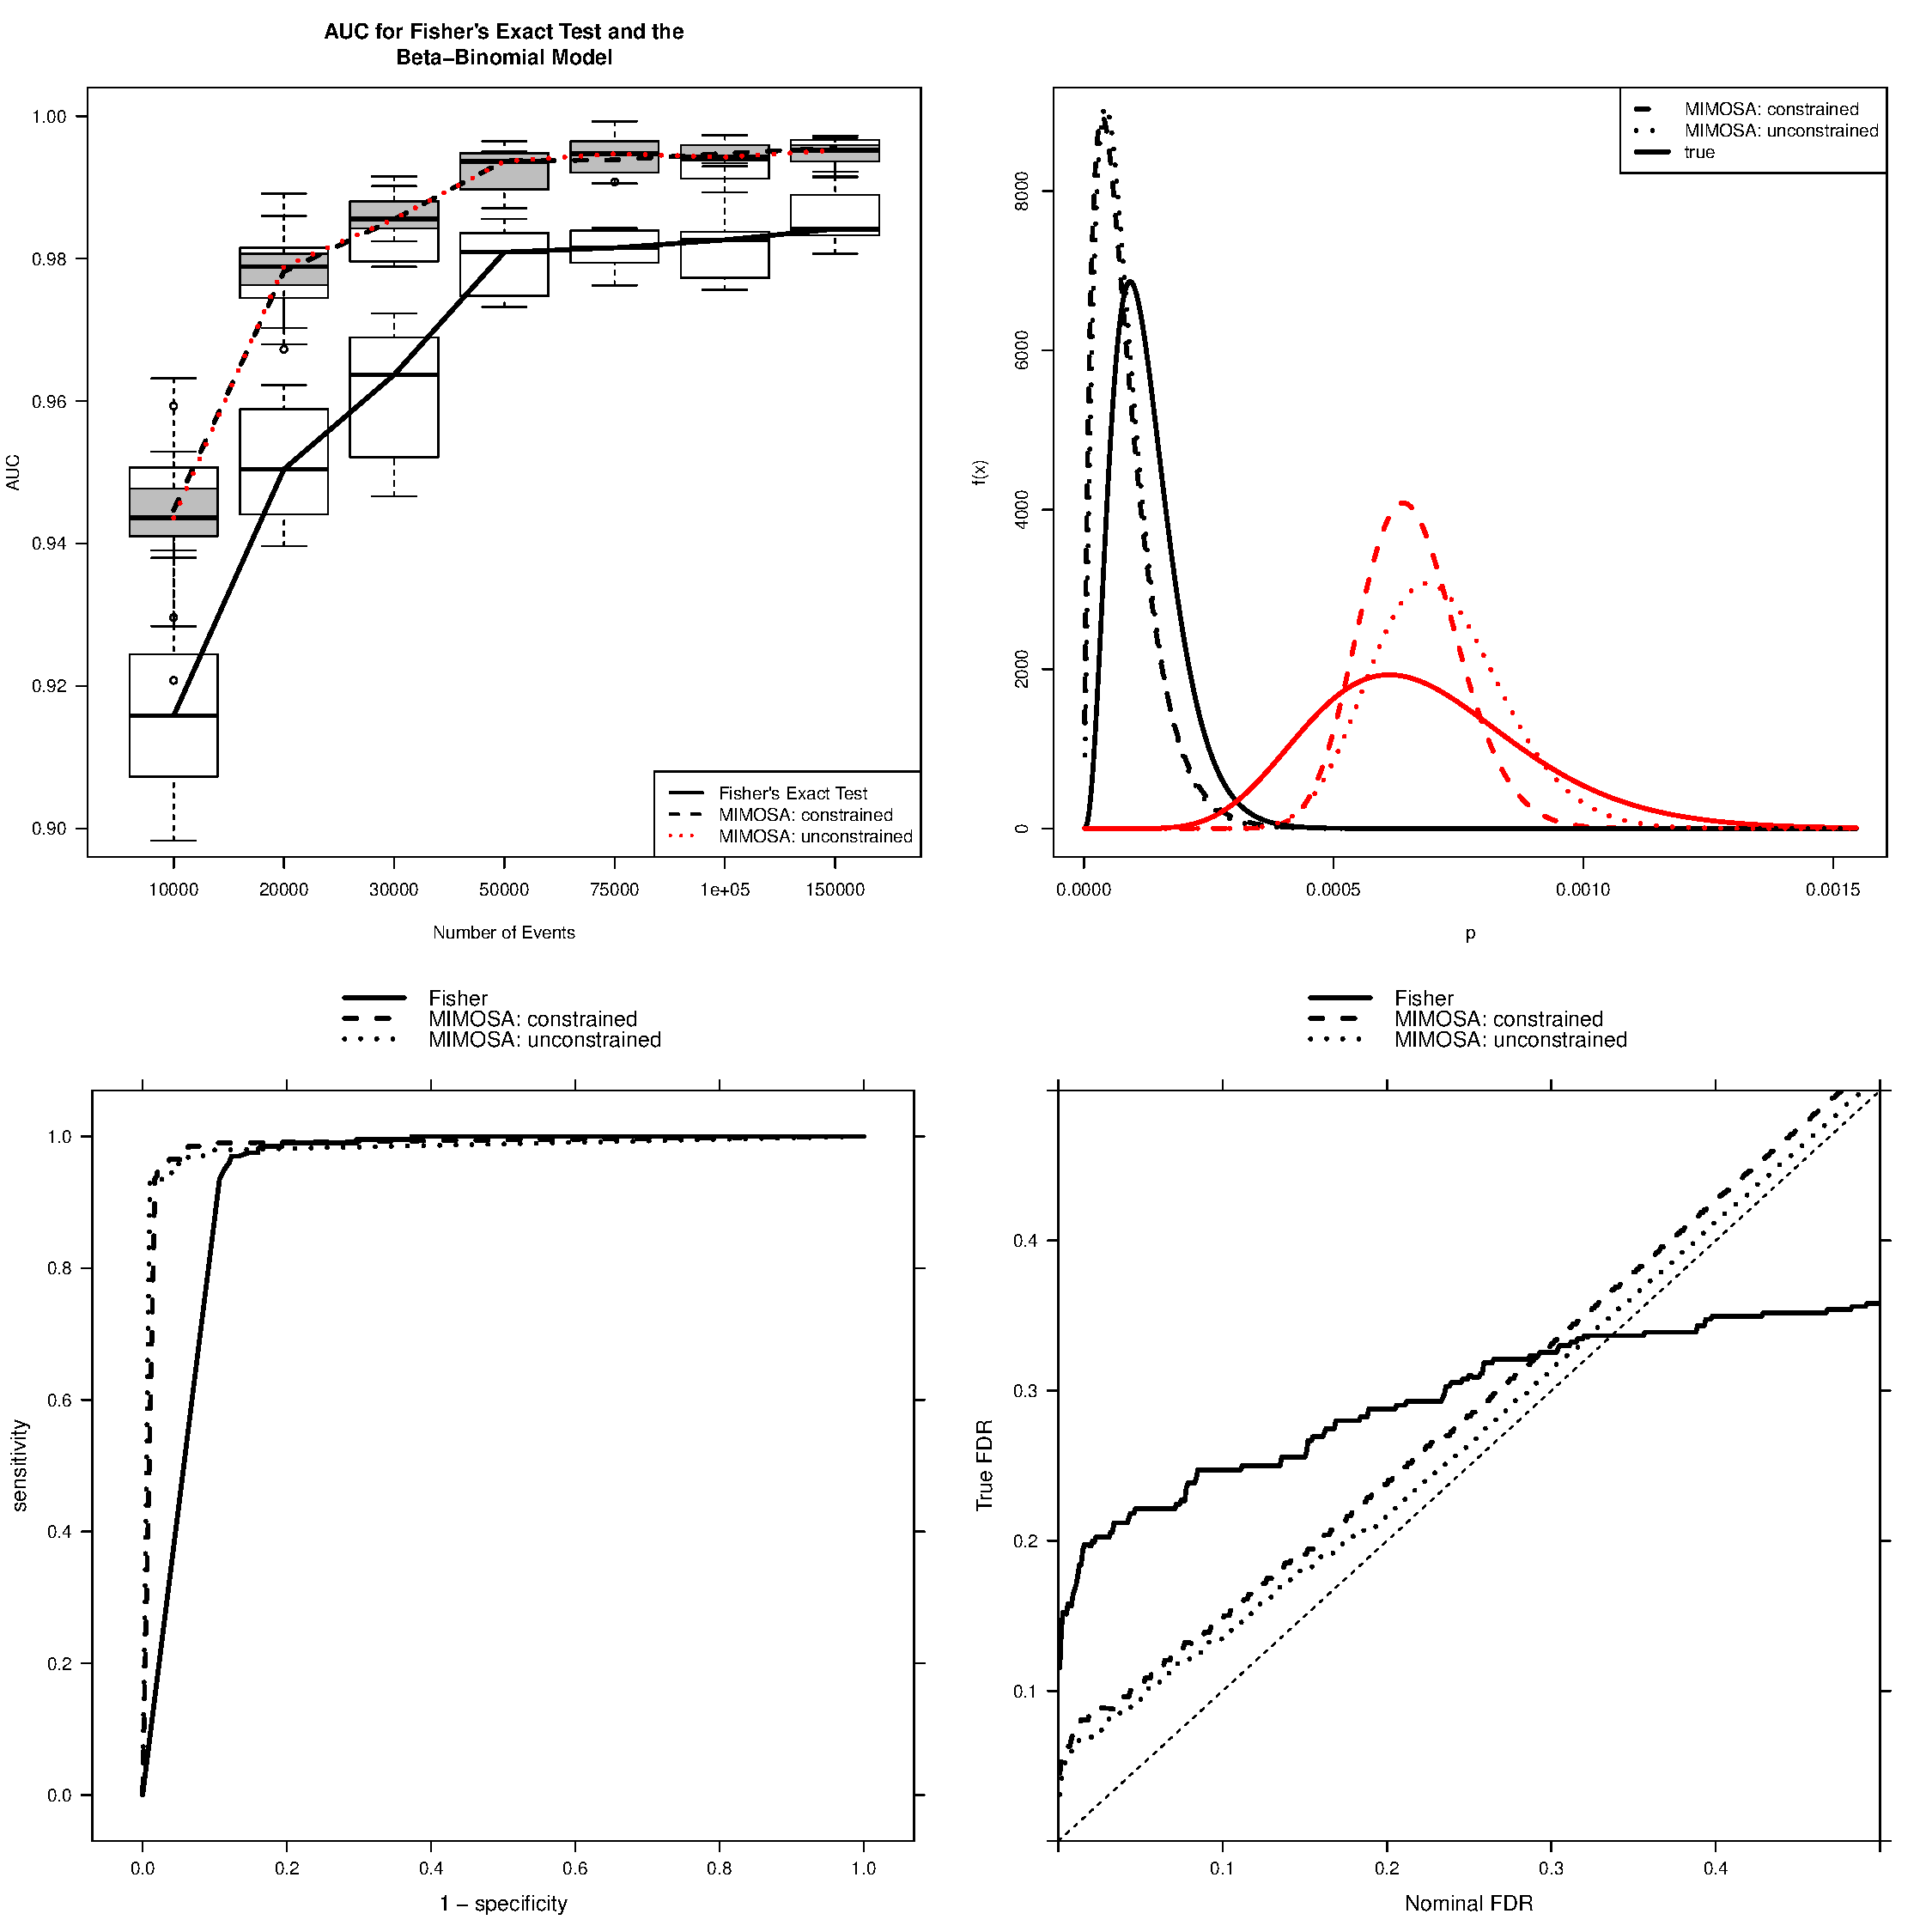
\includegraphics[width=4in]{Figures/simulations_all} 
   \caption{Performance of the constrained and unconstrained Beta--binomial mixture model vs Fisher's exact test on simulated data. Data were simulated from a constrained model with hyper--parameters estimated from a real data set of Gag1 stimulated, CD4+, IL2 expressing T--cells on day 28 from the HVTN054 trial. For total cell counts from 10,000 to 150,000, we simulated ten data sets each of 500 observations with a response rate of 40\%. The performance, measured by the AUC (area under the curve), of the constrained and unconstrained Beta--binomial mixture model compared to Fisher's exact test is shown in the first panel, as a function of increasing number of cells. The beta distributions for the estimated and true hyper parameters are shown in the second panel for one simulated data set, with N=150,000 events. The ROC curve for Fisher's exact test and the constrained and unconstrained Beta--binomial model for the same simulation are shown in the third panel. The observed vs expected false discovery rate for Fisher's exact test and the constrained and unconstrained Beta--binomial model are shown in the fourth panel.}
   \label{fig:simulations}
\end{figure}

\begin{figure}[htbp] %  figure placement: here, top, bottom, or page
   \centering
   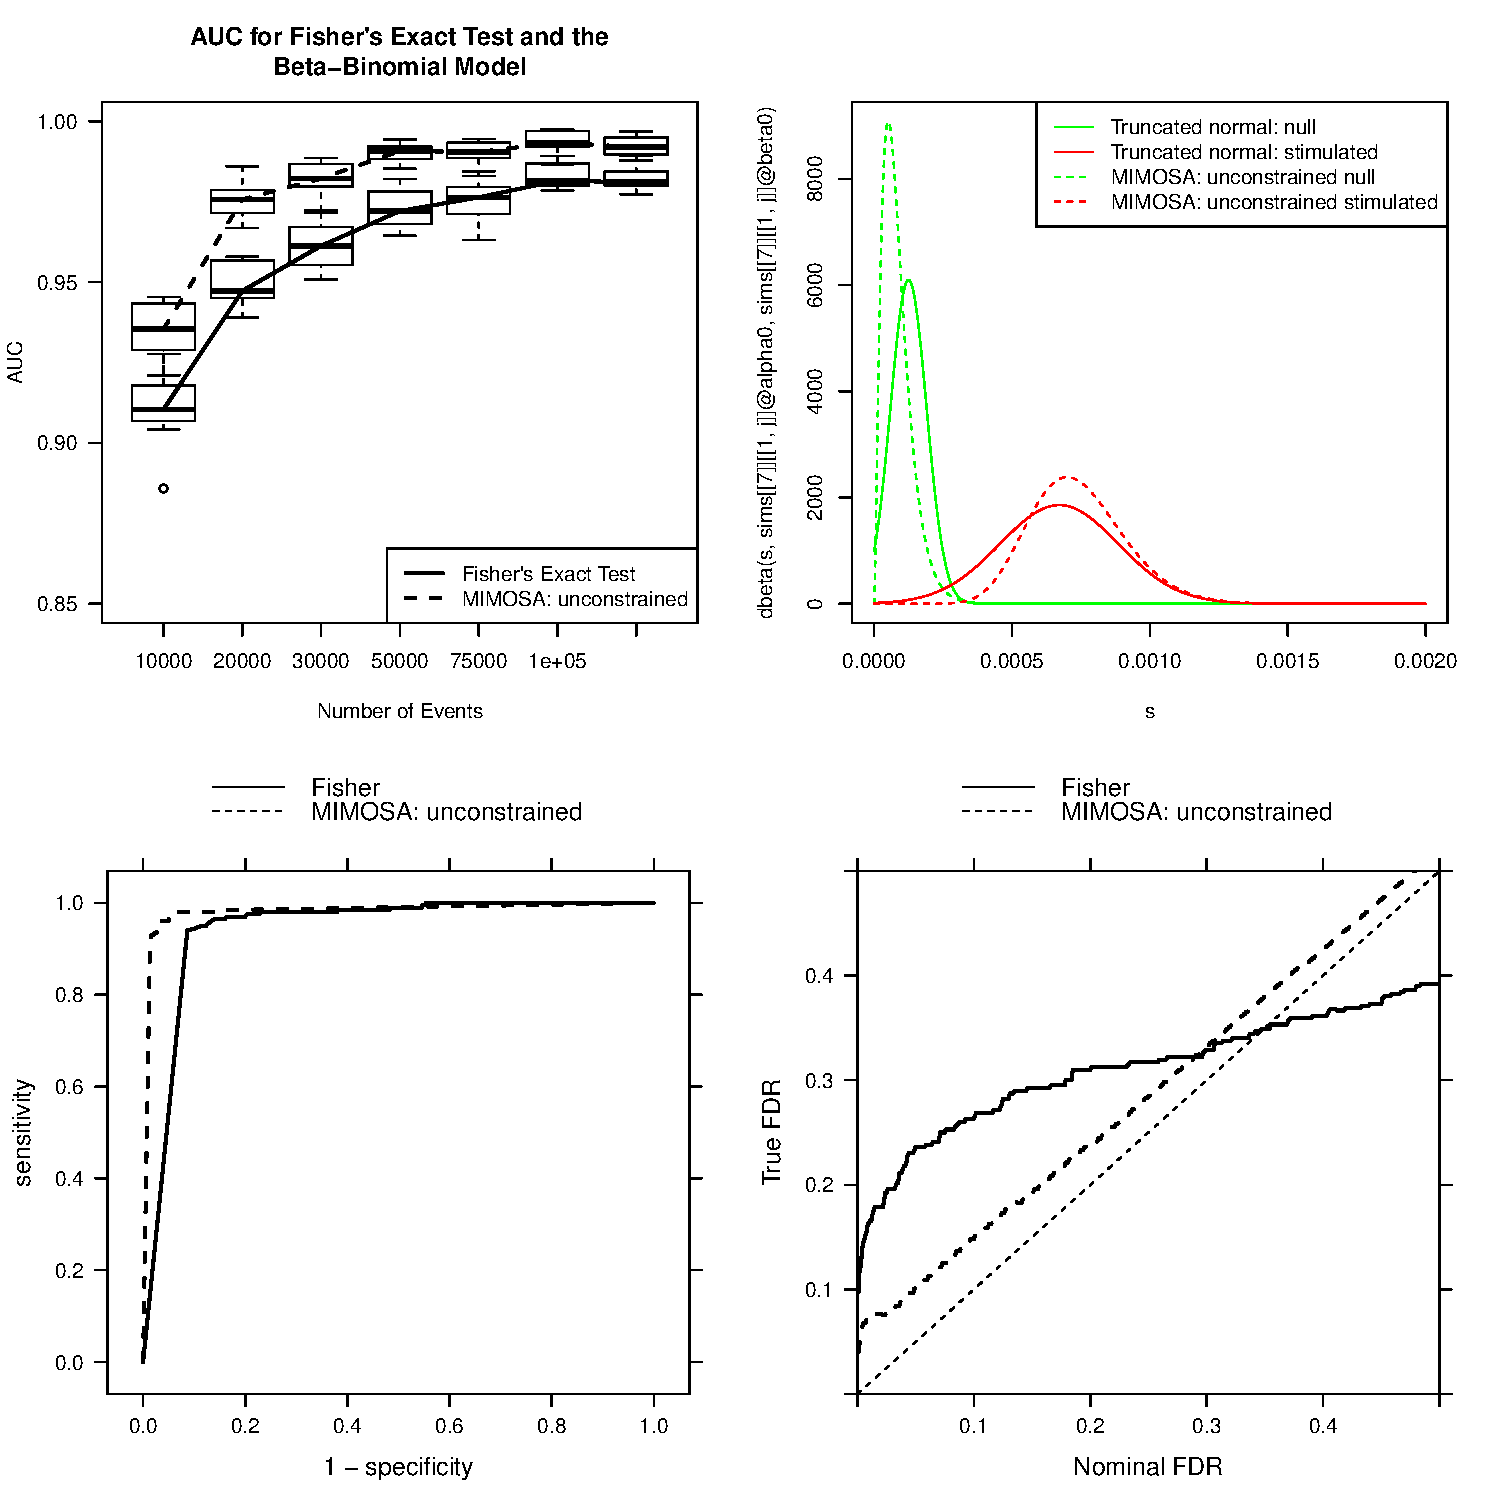
\includegraphics[width=4in]{Figures/simulations_violatedmodel} 
   \caption{Sensitivity to departures from model assumptions. We generated data from variant of the constrained model ($p_s>p_u$) where the proportions were simulated from truncated normal distributions on $(0,1)$, rather than from beta distributions. The mean and variance of the normal distributions was given by $\mu=\alpha/(\alpha+beta), \sigma^2=(\alpha\beta)/((\alpha+beta)^2(\alpha+\beta+1))$, where $\alpha,\beta$ are the Beta--prior hyper parameters for the MIMOSA model estimated from real data ($s, u$ subscripts omitted for brevity). The AUC for the unconstrained MIMOSA model and Fisher's exact test as a function of event count are shown in the first panel. The beta distributions for the estimated and true hyper parameters  are shown in the second panel. The ROC curves for one data set and the observed and true false discovery rates for the model and Fisher's exact test are shown in the third and fourth panels.}
   \label{fig:simulations_trunc}
\end{figure}


%\begin{figure}[htbp] %  figure placement: here, top, bottom, or page
%   \centering
%   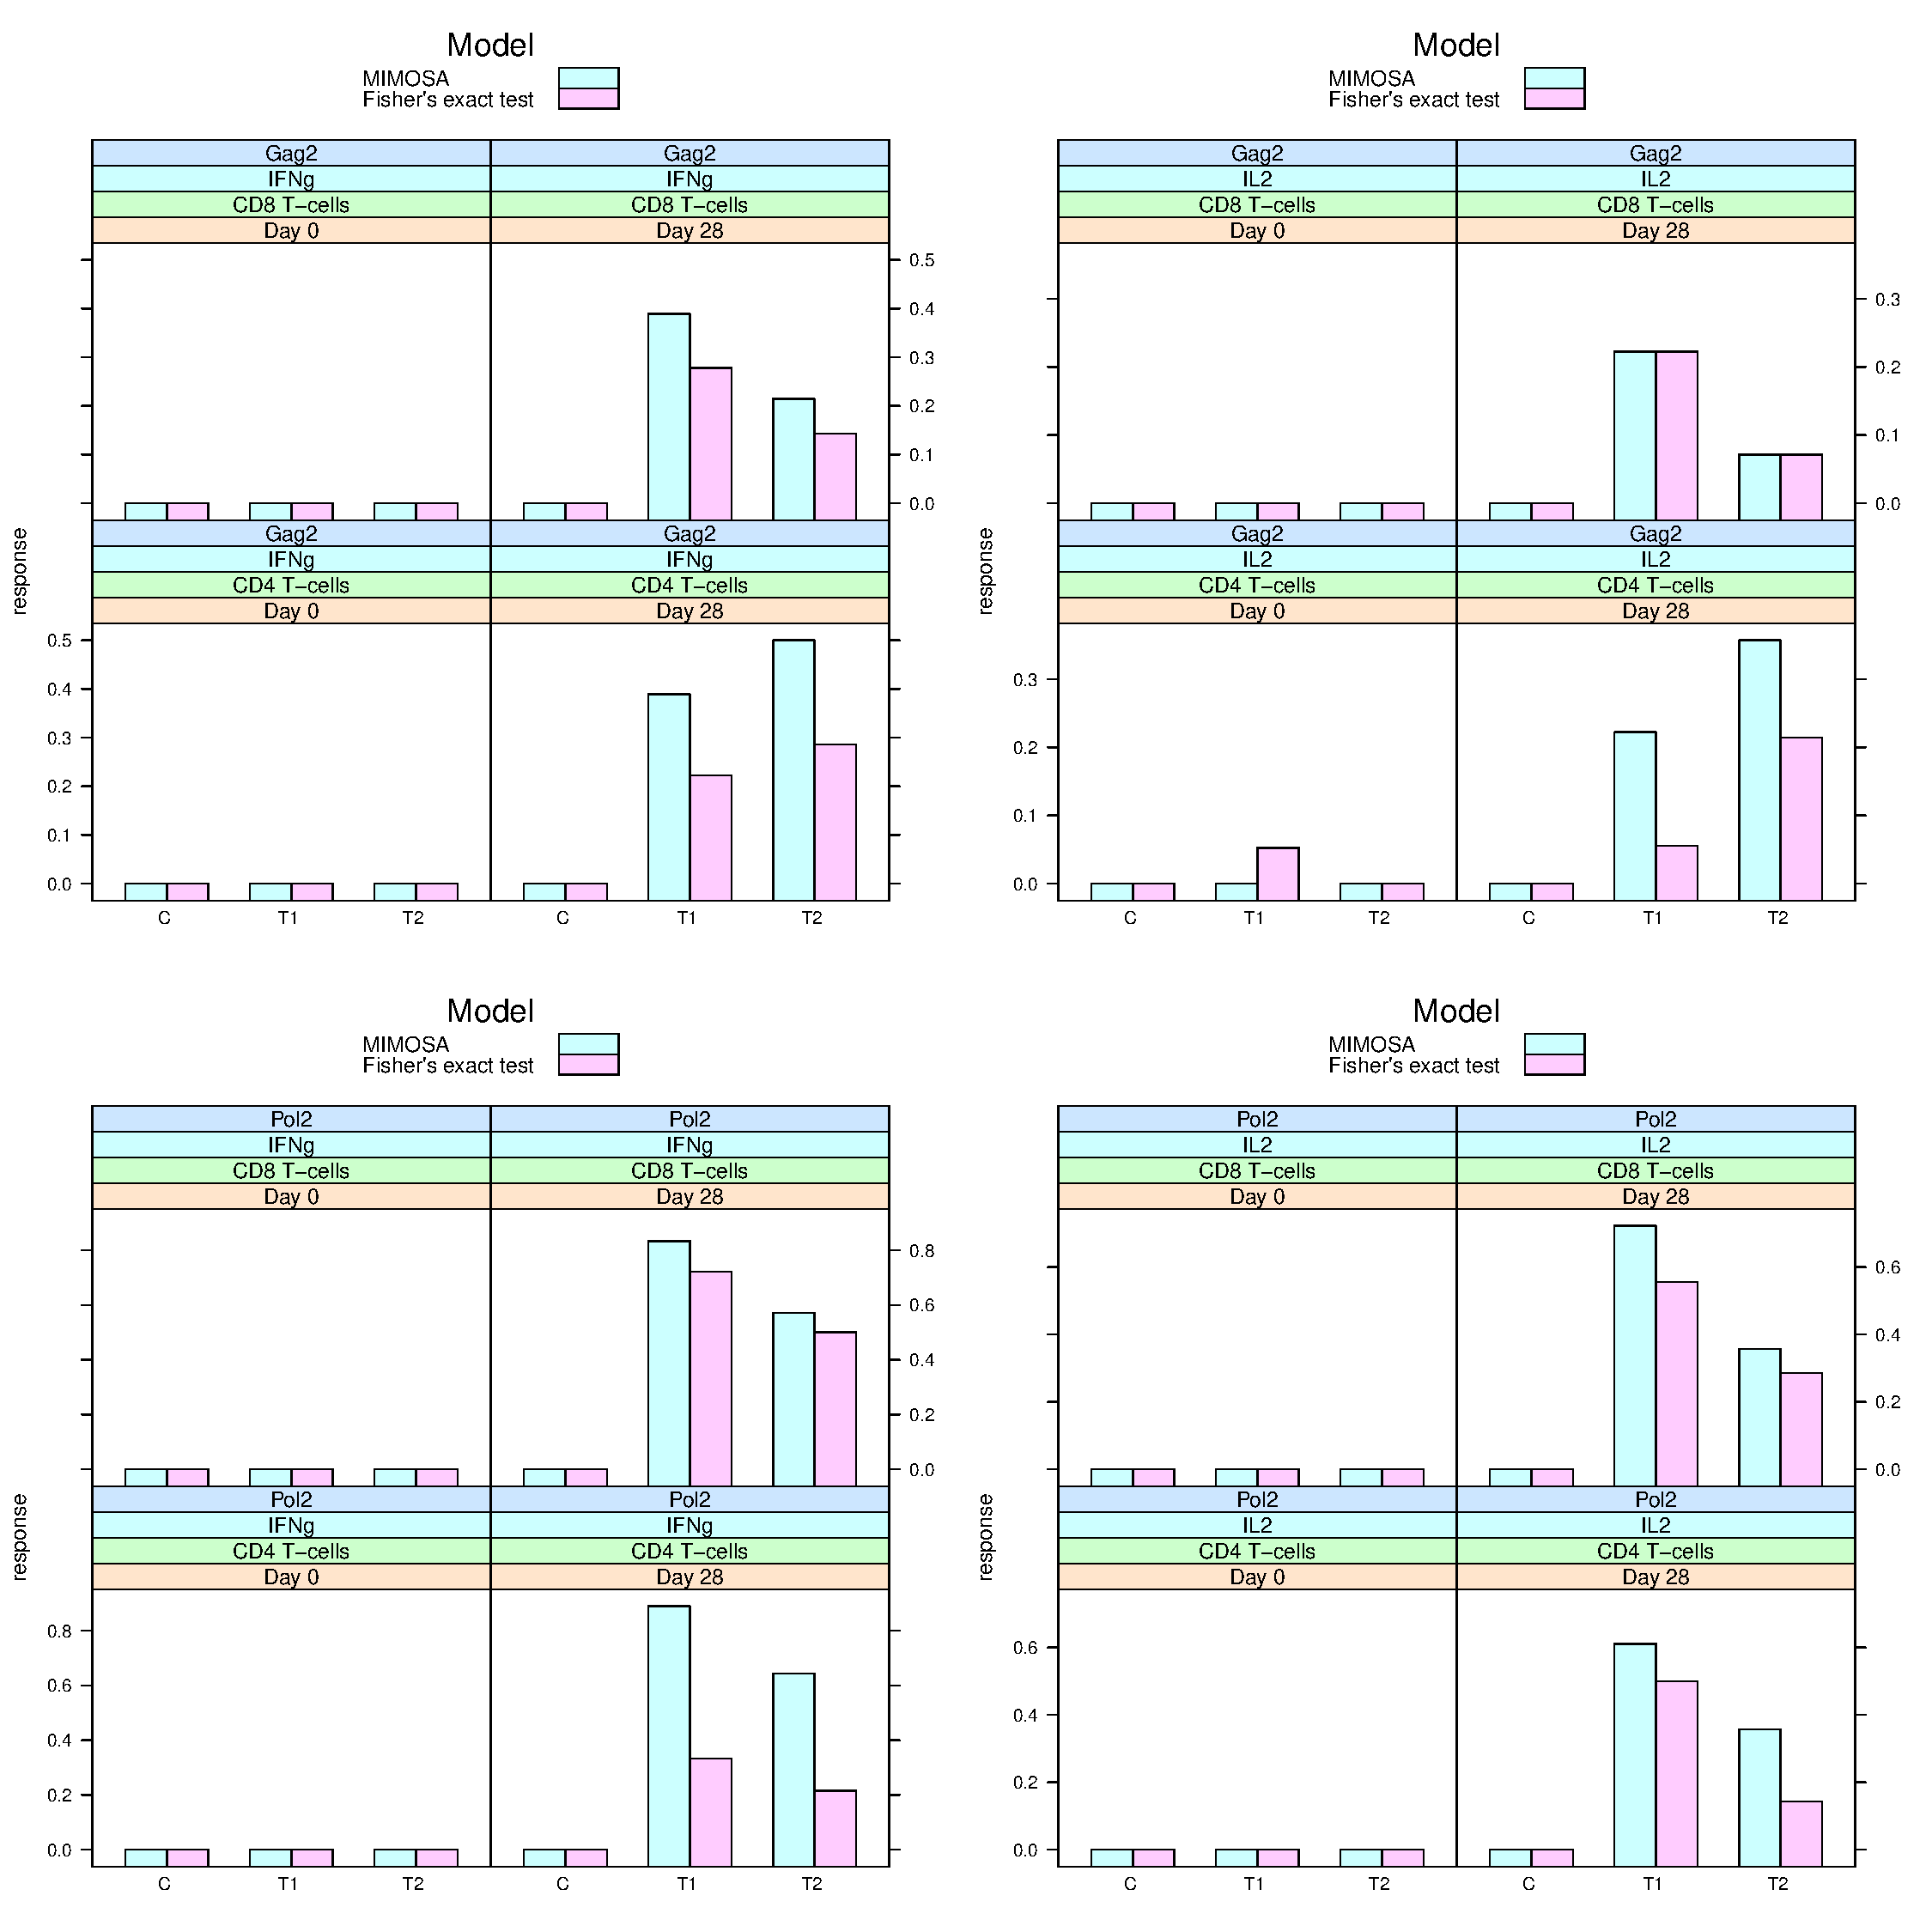
\includegraphics[width=6in]{Figures/PositivityRates} 
%   \caption{Comparison of MIMOSA and Fisher's exact test for calling responders in ICS data. Response rates for IL2 and IFNg cytokine positivity in Gag2 and Pol2 stimulated samples at days 0 and 28 in the CD4 and CD8 T--cell subpopulations of the HVTN054 ICS data. In the treatment groups, response rates for the MIMOSA model are greater than or equal to those for Fisher's exact test at day 28 but are equal (and zero) at day 0 as expected. In the control groups, response rates are equal (and zero) between Fisher's exact test and the MIMOSA model at day 0 and at day 28, as expected.}
%   \label{fig:positivityrates}
%\end{figure}

\begin{figure}[htbp] %  figure placement: here, top, bottom, or page
   \centering
   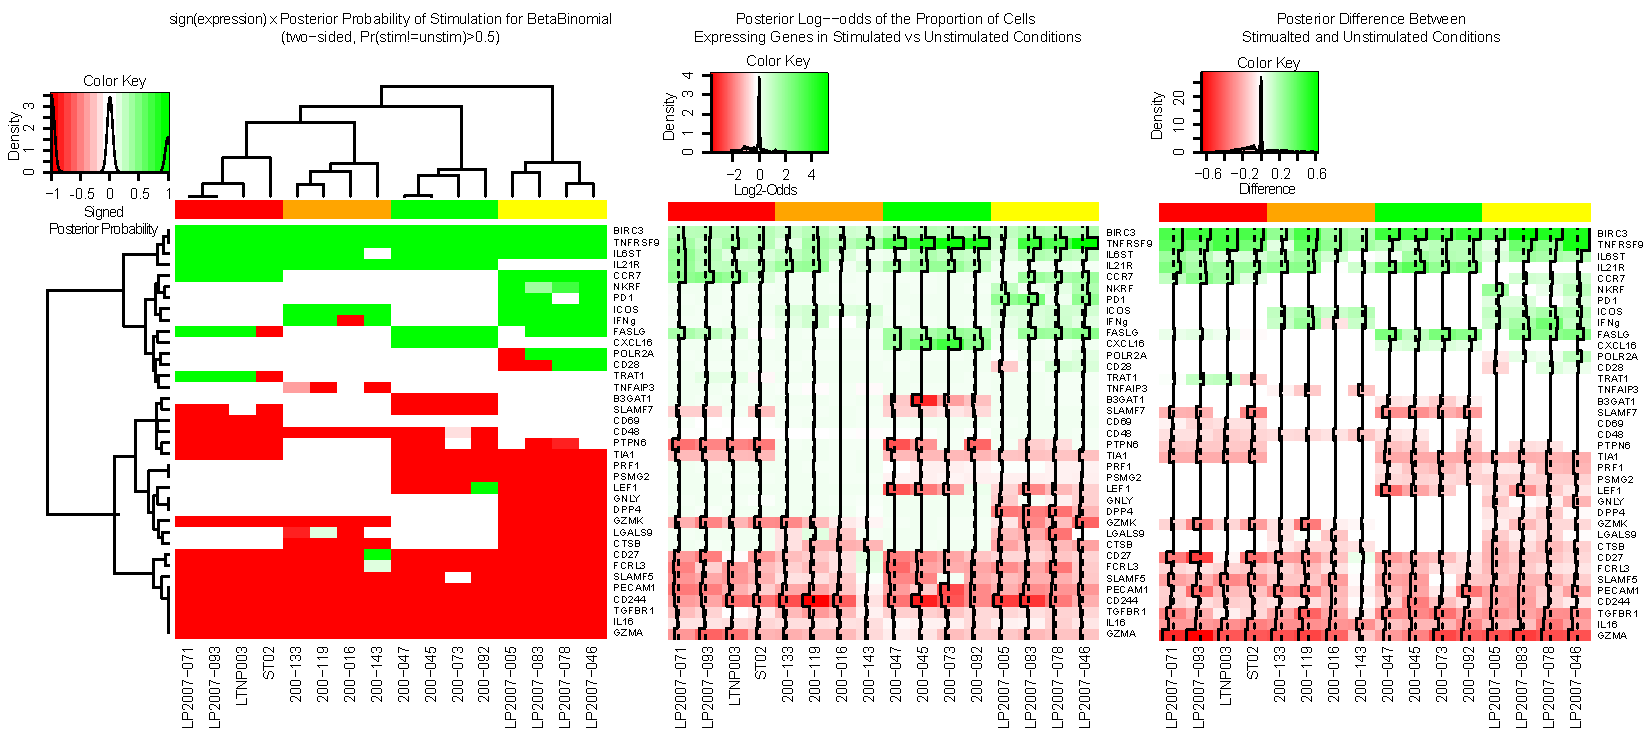
\includegraphics[width=6in]{Figures/FluidigmMIMOSA.pdf} 
  % \caption{Likelihood surface and volcano plot for IFNg producing, CD4+ T-cells in Gag2 stimulated vs control samples on day 28. A significant difference between control and stimulated samples is called at the 1\% FDR threshold (red) for the Beta--binomial model, and at 1\% for FDR adjusted p--values from Fisher's exact test (green). The likelihood surface shows the observed counts from stimulated and unstimulated samples. The volcano plot shows the difference between the proportion of cytokine positive cells in the stimulated and unstimulated samples, for the maximum likelihood estimates of the proportions (triangles) and for the MAP estimates (crosses). The effect of shrinking the MAP estimates towards zero can be seen in the volcano plot.}
%   \label{fig:icsdata}
\caption{Signed posterior probability, difference and log-odds ratio of the proportion of single cells expressing each gene on a 96x96 Fluidigm array. The posterior probability of response times the sign of the change in expression is shown in the first panel (red indicates a significant decrease, green a significant increase, relative to the control). Columns and rows are clustered based on these signed posterior probabilities. The middle panel shows the $log_2$ odds ratio of the proportion of cells expressing a gene in the stimulated vs. control samples. Rows and columns are ordered as in the left panel for comparison. The right panel shows the difference in the proportion of cells expressing each gene in the stimulated vs. control samples. Ordering of the rows and columns is preserved as in the first panel. The traces show the deviations of each cell from zero.}
\label{fig:fluidigm}
\end{figure}

\begin{figure}[htbp] %  figure placement: here, top, bottom, or page
   \centering
   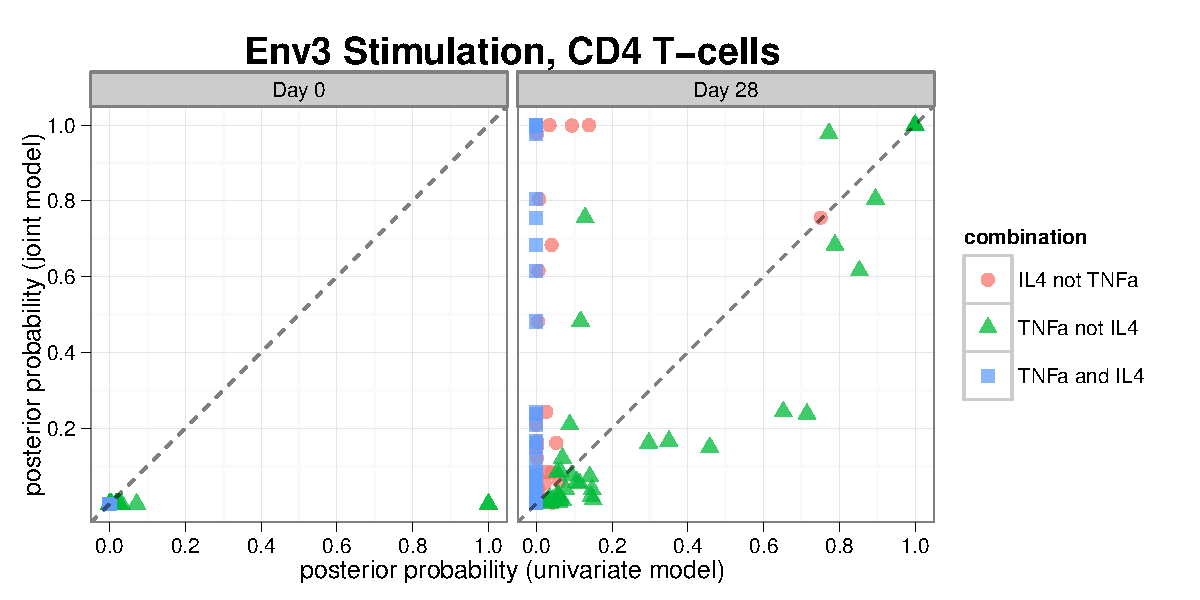
\includegraphics[width=6in]{Figures/Polyfunctionality_ggplot2} 
   \caption{Posterior probabilities from the four--dimensional, Multivariate--Dirichlet, MIMOSA model, compared against posterior probabilities from univariate MIMOSA for each combination of the cytokines IL4 and TNFa, on days zero and 28 for Env--2 peptide stimulated CD4+ T--cells.}
   \label{fig:polyfunctionality}
\end{figure}

\begin{figure}[htbp] %  figure placement: here, top, bottom, or page
   \centering
   \includegraphics[width=6in]{Figures/Polyfunctionality_Env1} 
   \caption{Posterior probabilities from the four--dimensional, Multivariate--Dirichlet, MIMOSA model, compared against posterior probabilities from univariate MIMOSA for each combination of the cytokines IL4 and TNFa, on days zero and 28 for Env--1 peptide stimulated CD4+ T--cells.}
   \label{fig:polyfunctionalityenv1}
\end{figure}


\renewcommand{\thesection}{S.\arabic{section}}
\renewcommand{\thesubsection}{\thesection.\arabic{subsection}}
\setcounter{section}{0}
\setcounter{subsection}{0}
%\todo[inline]{Note that the Supplementary Information section needs corrections to notation and overall}
\section*{Supplementary Information}
\section{Vaccine Trial ICS Dataset Description}
\label{supp:data}
HVTN054 is a phase 1 (safety and efficacy) trial of an adenoviral vector vaccine in individuals without prior immunity~\cite{Peiperl:2010ej}. The vaccine vector expressed Gag, Pol and Env proteins from multiple HIV clades~\cite{Peiperl:2010ej}. Vaccine was given at two increasing doses, as well as a placebo. T--cell responses to antigens in the vaccine were measured via the ICS assay~\cite{Peiperl:2010ej,Horton:2007tsa}. The cytokines measured were IFNg (Interferon--$\gamma$), IL2 (Interleukin--2), TNFa (Tumor necrosis factor--$\alpha$) and IL4 (Interleukin 4)~\cite{Horton:2007tsa}. The sample size consisted of 20 vaccine and four placebo recipients. The original statistical analysis of the positivity calls is described in the associated publication~\cite{Peiperl:2010ej}.
 
 
\section{Data Import, Preprocessing, and Gating}
The ICS assay data was imported into R from the original flowJo workspaces (version 6, TreeStar Inc, Ashland, OR)  using the BioConductor tool, \textit{flowWorkspace} (v 1.1.6) and ncdfFlow (v 1.1.4). Data were preprocessed using the flowJo--defined compensation matrices and data transformations extracted from the workspace file, and gated using methods from the flowCore package (v 1.19.2) to extract counts of cytokine positive and negative T--cells for each sample and stimulation~\cite{Hahne:2009vv}.

\section{Statistical Analysis in the Published Trial}
\label{supp:statpublished}
The methodology for statistical analysis and calling responders and non--responders in the original vaccine trial is described in the original publication~\cite{Peiperl:2010ej}. In general, a participant is called a ``responder'' to an antigen stimulation if, for a given cytokine, the number of cytokine--positive T-cells in the antigen--stimulated sample is significantly greater (for some statistical measure of significance) than the number of cytokine--positive T-cells for the negative control (unstimulated) sample from the same individual. In the original trial, significance was measured via one--sided Fisher's exact test for each participant and cytokine, comparing stimulated against unstimulated samples from that individual. In order to control the false positive rate for responder calls, made based on positivity for multiple cytokines, a discrete Bonferroni adjustment for multiple comparisons (across cytokines) was applied, and stimulations with an adjusted p--value below $\alpha = 0.00001$ were called positive~\cite{Horton:2007tsa}. 

%\subsection{Derivation of the Beta--Binomial Model for $p_s=p_u$ and $p_s>p_u$}
%\label{sec:derivation}
%
%We derive the posterior predictive distribution and marginal log--likelihood for the null model ($p_s=p_u$) and the alternative model ($p_s>p_u$) below: patient indices, $i$ on the $\left<N_s,n_s,N_u,n_u\right>$ are omitted for clarity. 
%For model \eqref{eq:null}, ($p_s=p_u, \alpha_s=\alpha_u, \beta_s=\beta_u$), the posterior predictive distribution of the data given the model is:
% \begin{align}
% 	\mathrm{Pr}(y_i|\alpha_u,\beta_u) &= \int\limits_{p_u=0}\limits^{1} \mathrm{Pr}(y_i,p_u|\alpha_u,\beta_u)dp_u\\
%	&=\int\limits_{p_u=0}\limits^{1} \mathrm{Pr}(y_i|p_u)\mathrm{Pr}(p_u|\alpha_u,\beta_u)dp_u\\
%	\begin{split}
%		=\int\limits_{p_u=0}\limits^{1}\binom{N_s+n_s}{n_s}p_u^{n_s}(1-p_u)^{N_s}\binom{N_u+n_u}{n_u}p_u^{n_u}(1-p_u)^{N_u}\cdot \\ 
%		\frac{1}{\mathrm{B}(\alpha_u,\beta_u)}p_u^{\alpha_u-1}(1-p_u)^{\beta_u-1}dp_u
%	 \end{split}\\
%	 \begin{split}
% 	=\binom{N_s+n_s}{n_s}\binom{N_u+n_u}{n_u}\frac{1}{\mathrm{B}(\alpha_u,\beta_u)}\cdot\\ \int\limits_{p_u=0}\limits^{1}p_u^{n_s+n_u+\alpha_u-1}(1-p_u)^{N_s+N_u+\beta_u-1}dp_u
%	\end{split}\\
%	\intertext{The integrand is the kernel of a beta distribution with parameters $\left(n_u+n_s+\alpha_u,N_u+N_s+\beta_u\right)$, giving a closed form expression for the  posterior predictive distribution of model \eqref{eq:null}:}
%	\mathrm{Pr}(y_i|\alpha_u,\beta_u)&=\binom{N_s+n_s}{n_s}\binom{N_u+n_u}{n_u}\frac{\mathrm{B}(n_s+n_u+\alpha_u,N_s+N_u+\beta_u)}{\mathrm{B}(\alpha_u,\beta_u)}\label{eq:model1postsupp}\\
%	\intertext{with marginal log--likelihood:}
%	\begin{split}
%	\mathcal{L}(\alpha_u,\beta_u|\mathbf{y})=\sum_{i=1}^P\left[\log{\binom{N^i_{s}+n^i_{s}}{n^i_{s}}}+\log{\binom{N^i_{u}+n^i_{u}}{n^i_{u}}}+\right.\\
%	\left.\log{\left(\mathrm{B}(n^i_s+n^i_u+\alpha_u,N^i_s+N^i_u+\beta_u)\right)}\right]-P\log\left(\mathrm{B}(\alpha_u,\beta_u)\right)\label{eq:model1MLLsupp}
%	\end{split}
% \end{align} 
% 
%For model \eqref{eq:alternate}, ($p_s>p_u$), the posterior predictive distribution of the data given the model is:
%\begin{align}
% 	\mathrm{Pr}(y_i|\alpha_u,\beta_u,\alpha_s,\beta_s) &= \int\limits_{p_u=0}\limits^1\int\limits_{p_s>p_u}\limits^{1} \mathrm{Pr}(y_i,p_u,p_s|\alpha_u,\beta_u,\alpha_s,\beta_s) dp_u  dp_s\label{eq:postpredmodel2}\\
%	\intertext{Assuming independence of stimulated and unstimulated observations in \eqref{eq:postpredmodel2}:} 
%	&=\int\limits_{p_u=0}\limits^{1}\int\limits_{p_s>p_u}\limits^1 \mathrm{Pr}(n_s|p_s)\mathrm{Pr}(n_u|p_u)\mathrm{Pr}(p_u|\alpha_u,\beta_u)\mathrm{Pr}(p_s|\alpha_s,\beta_s)dp_u dp_s\\
%		&=\int\limits_{p_u=0}\limits^{1}\mathrm{Pr}(n_u|p_u)\mathrm{Pr}(p_u|\alpha_u,\beta_u)dp_u \int\limits_{p_s>p_u}\limits^1 \mathrm{Pr}(n_s|p_s)\mathrm{Pr}(p_s|\alpha_s,\beta_s)dp_s\\
%		\begin{split}
%	=\int\limits_{p_u=0}\limits^{1}\left[ \binom{N_u+n_u}{n_u}p_u^{n_u}(1-p_u)^{N_u} \frac{1}{\mathrm{B}(\alpha_u,\beta_u)}p_u^{\alpha_u-1}(1-p_u)^{\beta_u-1}d p_u\right]\cdot \\ \int\limits_{p_s>p_u}\limits^{1}\left[ \binom{N_s+n_s}{n_s}p_s^{n_s}(1-p_s)^{N_s} \frac{1}{\mathrm{B}(\alpha_s,\beta_s)}p_s^{\alpha_s-1}(1-p_s)^{\beta_s-1}d p_s\right]
%	\end{split}\\
%	\begin{split}
%	 =\binom{N_u+n_u}{n_u} \binom{N_s+n_s}{n_s}\frac{1}{\mathrm{B}(\alpha_u,\beta_u)}\frac{1}{\mathrm{B}(\alpha_s,\beta_s)}\cdot\\
%	 \int\limits_{p_u=0}\limits^{1}\left[p_u^{n_u+\alpha_u-1}(1-p_u)^{N_u+\beta_u-1} d p_u\right]\int\limits_{p_s>p_u}\limits^{1}\left[p_s^{n_s+\alpha_s-1}(1-p_s)^{N_s+\beta_s-1}d p_s\right]
%	\end{split}
%	\end{align}
%	\begin{align}
%	\begin{split}
%	 =\binom{N_u+n_u}{n_u} \binom{N_s+n_s}{n_s}\frac{1}{\mathrm{B}(\alpha_u,\beta_u)}\frac{1}{\mathrm{B}(\alpha_s,\beta_s)}\cdot\\
%	 \int\limits_{p_u=0}\limits^{1}\left[p_u^{n_u+\alpha_u-1}(1-p_u)^{N_u+\beta_u-1}d p_u \right]\left(1-\int\limits^{p_u}\limits_{p_s=0}\left[p_s^{n_s+\alpha_s-1}(1-p_s)^{N_s+\beta_s-1}d p_s\right]\right)
%	\end{split}
%	\intertext{The second integral can be expressed as the CDF of the beta distribution, also known as the regularized incomplete beta function, $\mathrm{I}_x(\alpha,\beta)$}
%	\begin{split}
%	 =\binom{N_u+n_u}{n_u} \binom{N_s+n_s}{n_s}\frac{1}{\mathrm{B}(\alpha_u,\beta_u)}\frac{\mathrm{B}(n_s+\alpha_s,N_s+\beta_s)}{\mathrm{B}(\alpha_s,\beta_s)}\cdot\\
%	 \int\limits_{p_u=0}\limits^{1}\left[p_u^{n_u+\alpha_u-1}(1-p_u)^{N_u+\beta_u-1} \right]\left(1-\mathrm{I_{p_s}}(n_s+\alpha_s,N_s+\beta_s)\right)d p_u
%	\end{split}\\
%	\intertext{giving the posterior predictive distribution of model \eqref{eq:alternate}}
%	\begin{split}
%		 =\binom{N_u+n_u}{n_u} \binom{N_s+n_s}{n_s}\frac{\mathrm{B}(n_u+\alpha_u,N_u+\beta_u)}{\mathrm{B}(\alpha_u,\beta_u)}\frac{\mathrm{B}(n_s+\alpha_s,N_s+\beta_s)}{\mathrm{B}(\alpha_s,\beta_s)}\cdot\\
%	 \int\limits_{p_u=0}\limits^{1}\left[\frac{1}{\mathrm{B}(n_u+\alpha_u,N_u+\beta_u)}p_u^{n_u+\alpha_u-1}(1-p_u)^{N_u+\beta_u-1} \right]\left(1-\mathrm{I_{p_u}}(n_s+\alpha_s,N_s+\beta_s)\right)d p_u\label{eq:model2postsupp}
%	\end{split}
%\end{align}
%The integral in equation~\eqref{eq:model2postsupp} is computed numerically. The marginal log--likelihood of model~\eqref{eq:alternate} is then:
%\begin{equation}
%		 \begin{split}
%		 \mathcal{L}(\alpha_s,\alpha_u,\beta_s,\beta_u|\mathbf{y})=-P\log\left(\mathrm{B}(\alpha_u,\beta_u)\right)-P\log\left(\mathrm{B}+(\alpha_s,\beta_s)\right)+\\ \sum_{i=0}^P\left\{\log\binom{N^i_u+n^i_u}{n^i_u}+ \log\binom{N^i_s+n^i_s}{n^i_s}+ \log\left(\mathrm{B}(n^i_u+\alpha_u,N^i_u+\beta_u)\right)+ \log\left(\mathrm{B}(n^i_s+\alpha_s,N^i_s+\beta_s)\right)+\right. \\ \left. \log\left(\hspace{1em}\int\limits_{p_u=0}\limits^{1}\left[\frac{1}{\mathrm{B}(n^i_u+\alpha_u,N^i_u+\beta_u)}p_u^{n^i_u+\alpha_u-1}(1-p_u)^{N^i_u+\beta_u-1} \right]\left(1-\mathrm{I_{p_u}}(n^i_s+\alpha_s,N^i_s+\beta_s)\right)d p_u\right)\right\}\label{eq:model2MLLsupp}
%\end{split}
%\end{equation}
%\subsection{The Beta-Binomial Mixture Model}
%For a given stimulation, not all individuals are expected to exhibit an immune response to that stimulation. Therefore, for a set of ICS data, any single observation, ($n^i_s,n^i_u$) could either be derived from model~\eqref{eq:null}, or from model~\eqref{eq:alternate}. We model this situation explicitly using a mixture--model framework.
\clearpage
\bibliographystyle{unsrtnat}
\bibliography{MIMOSA}

\end{document}  
